\documentclass{article}

\usepackage[T1,T2A]{fontenc}
\usepackage[utf8]{inputenc}
\usepackage[english,russian]{babel}

\usepackage{pdfpages}
\usepackage{multirow}

\usepackage{caption}

\usepackage{amsmath}
\usepackage[hidelinks]{hyperref}


\usepackage{graphicx}%Вставка картинок
\graphicspath{{noiseimages/}}

\usepackage{float}%'Плавающие' картинки
\usepackage{wrapfig}%Обтекание фигур (таблиц, картинок и прочего)

% Параграфы перед главами, но их не будет перед сабсекциями
\renewcommand{\thesection}{\S\arabic{section}}
\renewcommand{\thesubsection}{\arabic{section}.\arabic{subsection}}

\makeatletter
\def\@biblabel#1{#1. }
\makeatother

\setlength{\emergencystretch}{10pt}

\begin{document}

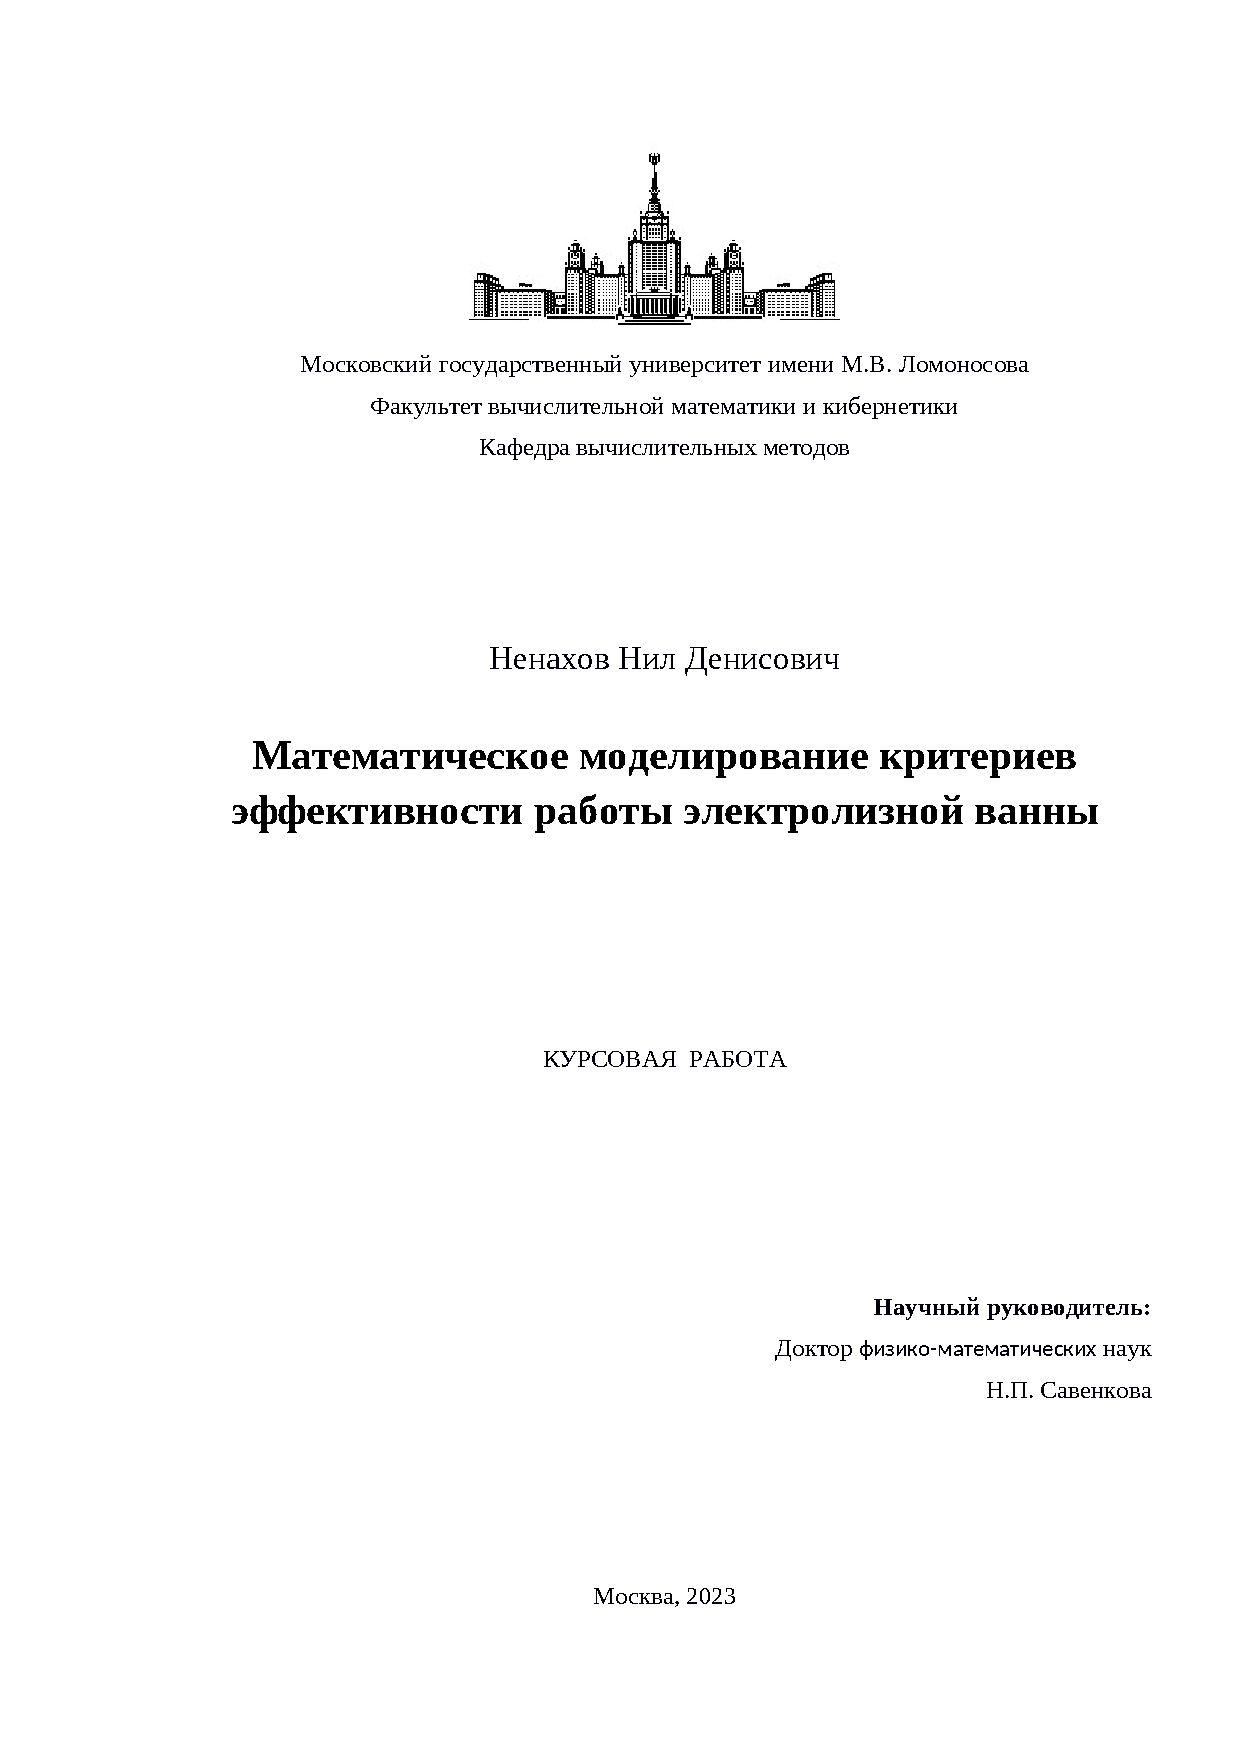
\includepdf[pages=-]{Titul.pdf}

\newpage

% переименовываем  список литературы
\addto\captionsrussian{\def\refname{Список литературы}}

\setcounter{tocdepth}{5}
\tableofcontents

\newpage

\section*{Введение.}
\addcontentsline{toc}{section}{Введение}

\subsection*{Постановка задачи.}
\addcontentsline{toc}{subsection}{Постановка задачи}

Целью исследовательской работы является проведение математического моделирования одного из основных параметров процесса промышленного электролиза алюминия — потери выхода алюминия по току.

Производство алюминия играет очень важную роль в экономике России. Процесс электролиза очень сложен, энергозатратен и серьезно влияет на экологию. Для удешевления себестоимости металла и улучшения экологичности производства имеет смысл совершенствовать не только устройство электролизера, но и способы управления процессом электролиза. С этой целью в промышленных цехах производства алюминия создаются линии АСУТП (автоматическая система управления технологическим процессом), которые позволяют значительно повысить эффективность принятия решений при управлении процессом электролиза с целью повышения выхода алюминия и исключения негативного влияния человеческого фактора.

АСУТП, ориентируясь на значения управляющих параметров, автоматически оценивают текущее состояние процесса электролиза и принимают управляющие решения по стабилизации и повышению эффективности процесса электролиза. В силу высокой температуры и агрессивности среды использование большинства приборов становится практически невозможно. В настоящее время расчет управляющих параметров происходит на основе полуэмпирических формул, в которые входят значения, которые получаются в результате физико-физических экспериментов (замеров), проводимых в реальном времени~\cite{litlink:kalmykov}. В отдельных случаях некоторые химические характеристики рассчитываются на основе одномерных математических моделей, большинство из которых не являются динамическими. Замер межполюсного расстояния и химический анализ состава электролита измеряется раз в две недели, поэтому АСУТП вынуждена принимать управляющие решения на основе устаревших данных по этим управляющим параметрам. Регулярно измеряются лишь несколько параметров: это сила тока и напряжение в рабочем пространстве электролизера, также могут быть измерены падение напряжения на аноде и в ошиновке~\cite{litlink:bibliogr}.

Целью данной работы является проведение математического моделирования одного из основных параметров производства алюминия — потери выхода алюминия по току — в целях повышения эффективности работы АСУТП.

\subsection*{Обзор литературы.}
\addcontentsline{toc}{subsection}{Обзор литературы}

Ниже приведено краткое описание процесса электролиза алюминия и основных типов алюминиевых электролизеров~\cite{litlink:bibliogr}.

Процесс получения алюминия электролизом глинозема происходит по следующей схеме. В прямоугольную ванну, футерованную углеродистым материалом, помещается слой расплавленного алюминия, над ним - слой расплавленного глинозема. В ванну опускают один анод (в случае электролизера Соделберга), через который поступает электрический ток в рабочее пространство ванны. В качестве побочного продукта образуются газы ($CO, CO_2$), которые скапливаются под анодом~\cite{litlink:bibliogr}. Схема алюминиевого электролизера приведена на рисунке \ref{fig:elec}.

Электролизеры с самообжигающимся анодом (электролизеры Соделберга) имеют один анод и уступают многоанодным ваннам в производительности и экологичности. В свою очередь для многоанодных электролизеров требуются заранее изготовленные аноды, которые попарно заменяются после выработки текущих. Используемая сила тока напрямую зависит от типа и конструкции электролизера и может варьироваться от 70 кА до 400 кА при напряжении в 4-5 В~\cite{litlink:bibliogr}.

\begin{figure}[H]
	\centering
	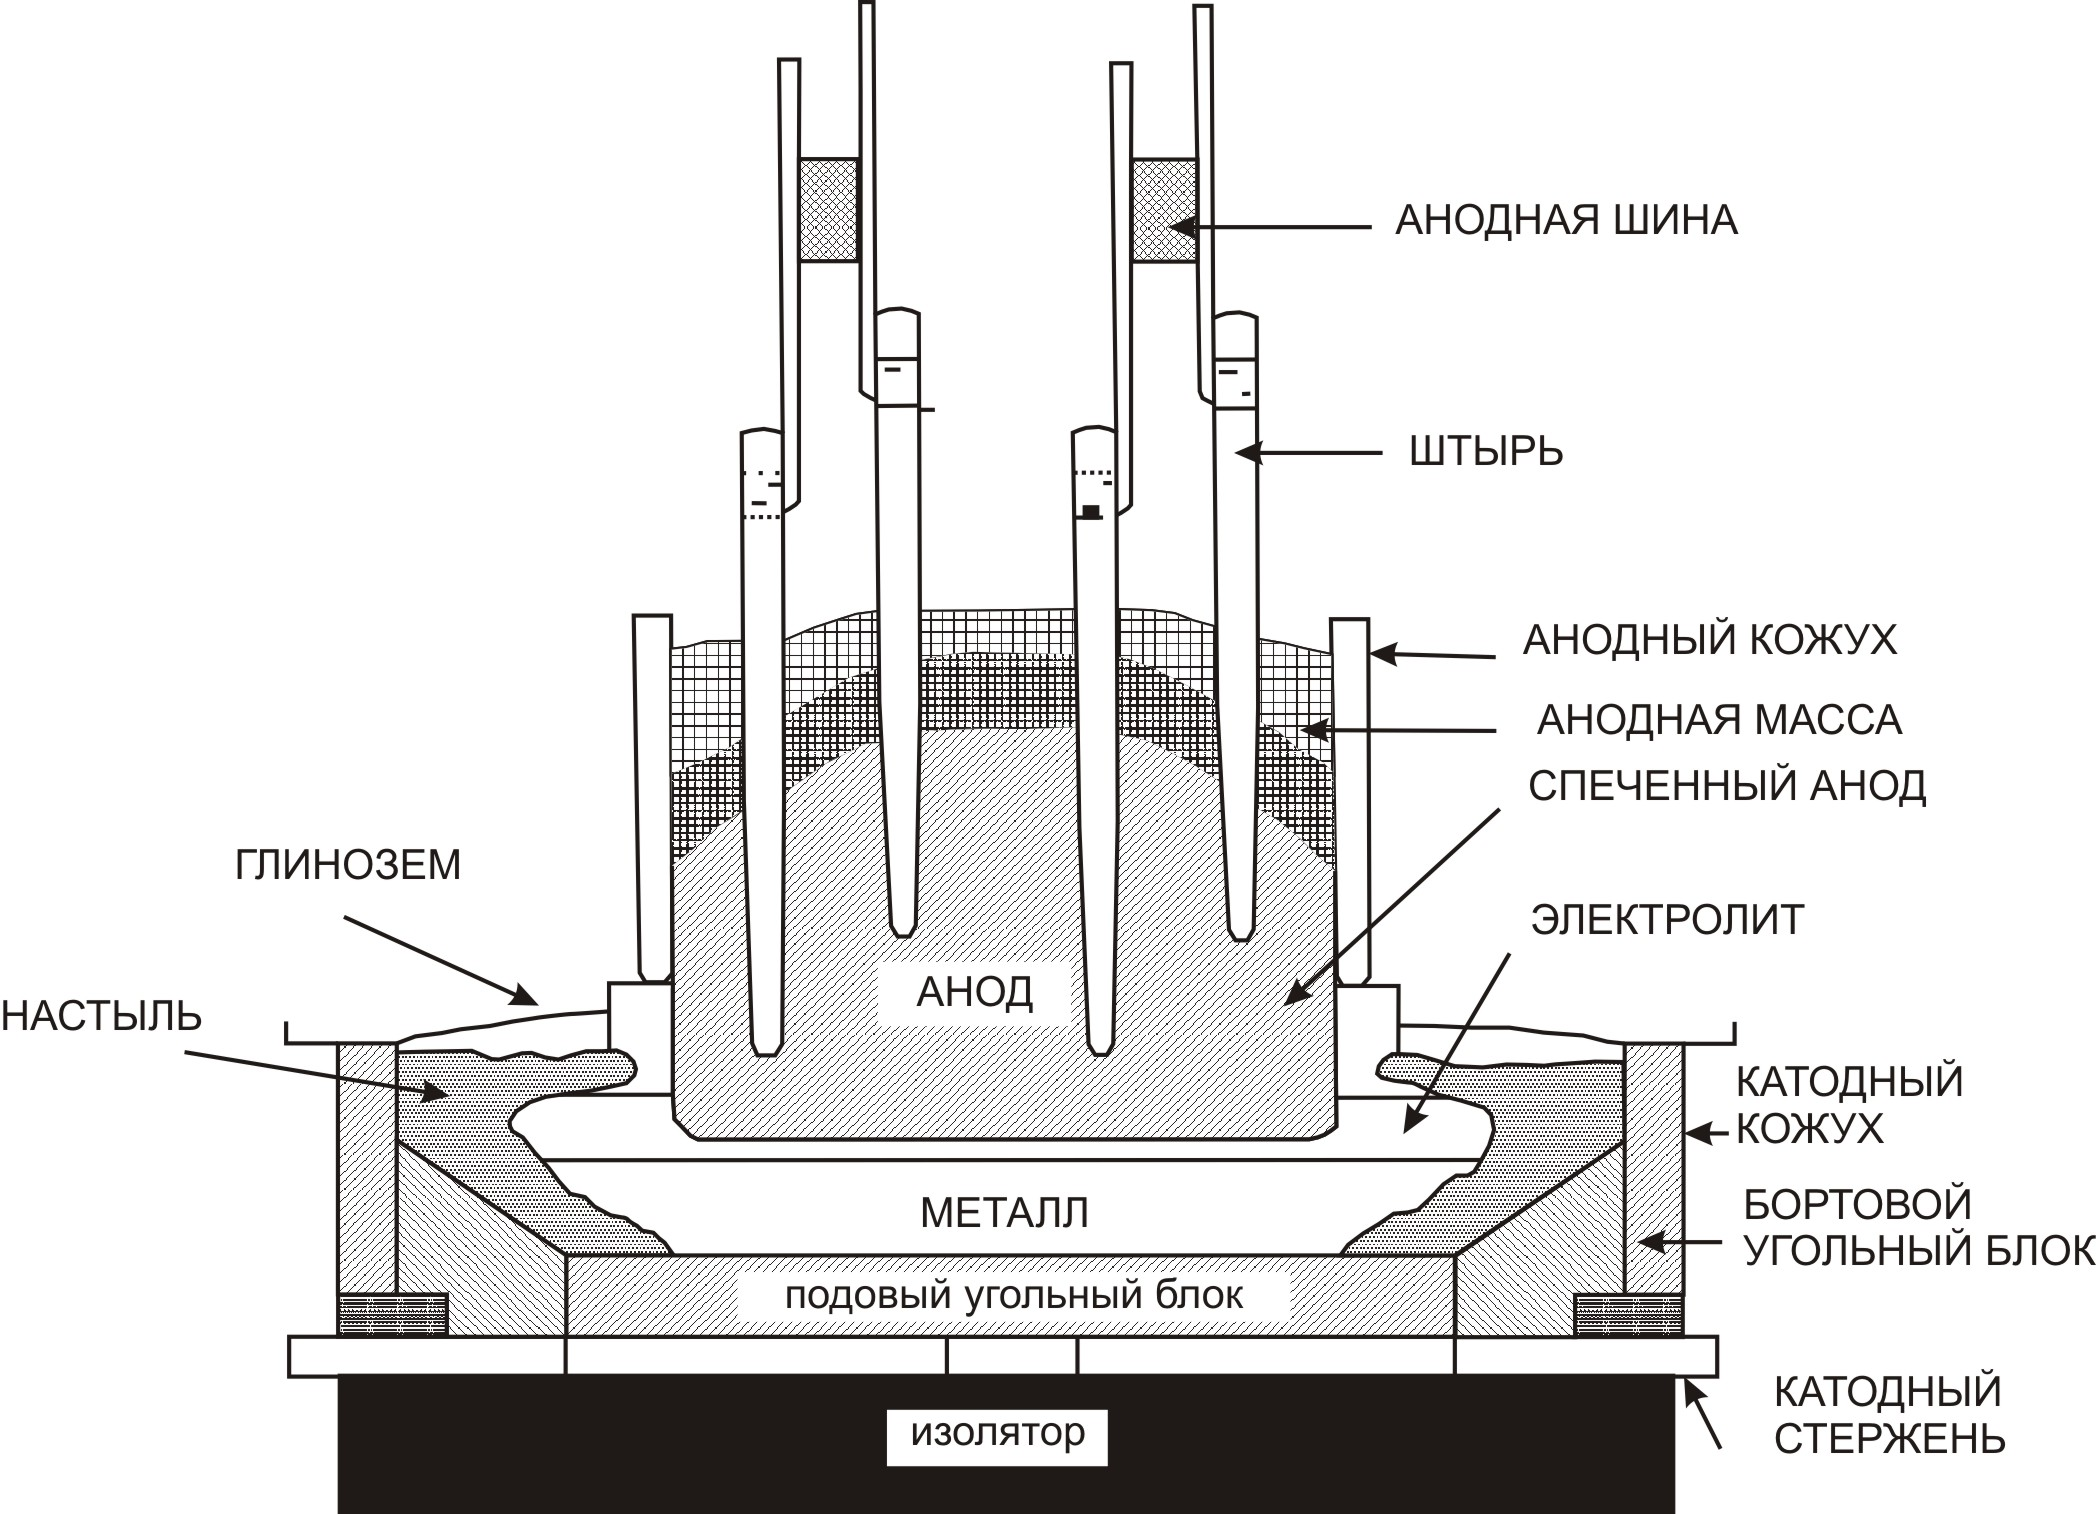
\includegraphics[width=0.8\linewidth]{Electrolizer.jpg}
	\caption[]{}
	\label{fig:elec}
	Поперечный разрез алюминиевого электролизера с самообжигающимся анодом.
\end{figure}

Работу, которую совершает ток при прохождении через ванну, можно вычислить по формуле
\begin{equation}
 A=U \cdot I \cdot t,
\end{equation}
где U - напряжение на электролизере, I - сила тока, t - время (см.~\cite{litlink:derkach}).

Теоретическое количество алюминия, которое должно получиться при электролизе, вычисляется по закону Фарадея
\begin{equation}\label{eq:faradey}
M=F \cdot I \cdot t.
\end{equation}

При этом количество реального произведенного металла всегда несколько меньше теоретического значения и вычисляется по формуле 
\begin{equation}\label{eq:real}
P=\eta \cdot F \cdot I \cdot t,
\end{equation}
где $\eta$ - выход по току, F - константа Фарадея (см.~\cite{litlink:derkach}).

Для оценки эффективности производства необходимо связать количество полученного алюминия с затраченной энергией (удельный расход энергии)
\begin{equation}
W=\frac{A}{P}=\frac{U}{F \cdot \eta}.
\end{equation}
Обычно это величина колеблется от 12,5 до 18,0 кВт$\cdot$ч/кг. 

Из формул (\ref{eq:faradey}) и (\ref{eq:real}) следует, что
\begin{equation*}
\eta=\frac{P}{M},
\end{equation*}
где $\eta$ выход по току (безразмерный управляющий параметр).

На практике часто используют величину процентного выхода по току
\begin{equation}
\eta=\frac{100 \cdot P}{M}.
\end{equation}

Выход по току зависит от большого числа параметров: температуры, межполюсного расстояния (МПР), плотности тока, состава электролита, криолитового отношения (КО), конструкции, геометрии электролизеров, электромагнитных сил.

Перечислим основные физико-химические процессы, проходящие в электролизной ванне~\cite{litlink:kalmykov}, которые активно влияют друг на друга:
\begin{itemize}
\item гидродинамические процессы,
\item электромагнитные процессы,
\item химические процессы,
\item тепловые процессы
\end{itemize}

Гидродинамические процессы определяют циркуляцию вещества в расплаве электролита и в расплаве металла. Поскольку сырье в электролизер подается точечно, то распределение скоростей в электролите отвечает за перенос сырья в рабочем пространстве ванны. Неравномерное распределение загруженного в ванну глинозема ведет к потери выхода алюминия по току~\cite{litink:AE}.

Магнитогидродинамические процессы, возникающие во время прохождения тока через электролизер, сильно влияют на МГД (магнитогидродинамическую) стабильность ванны.

Температура алюминия и подины также серьезно влияют на процесс производства, при снижении температуры расплава возможно образование коржей, которые уменьшают рабочую поверхность подины. В свою очередь, слишком высокая температура приводит к расплавлению защитного слоя на боковых стенках ванны в зоне раздела металла.

Самым общим показателем эффективности управления процессом получения алюминия является себестоимость производства алюминия. Однако этот критерий зависит от большого числа параметров, никак не связанных с самим процессом электролиза. Поэтому вводятся другие параметры, приближенные к технологическому процессу. Это расход электроэнергии на тонну получаемого металла, удельный расход углерода и удельный расход фторидов. Эти управляющие параметры зависят друг от друга, однако их соотношения могут меняться в зависимости от специфики конкретного производства.

В ВАМИ (Всероссийский Алюминиево-магниевый Институт) была получена эмпирическая формула для расчета практического выхода по току~\cite{litlink:VAMI}
\begin{equation} \label{eq1}
\eta=(1-2567 \cdot \frac{S^{0,21}_{anod}}{i^{0.58}_a \cdot L_{ACD} \cdot e^{\frac{12940}{T_e}}}) \cdot 100,
\end{equation}
где $i_a$ - анодная плотность тока, $S_{anod}$ - площадь анода, $L_{ACD}$ - МПР, $T_e$ - температура электролита.

В работе~\cite{litlink:korobov} предложено следущее эмпирическая формула для расчета практического выхода алюминия:
\begin{equation} \label{eq:p}
P= \frac{wT-920}{0.336 \cdot \eta \cdot b}[0.112+\frac {1.12}{\delta \cdot (h+30)}+0.056 \cdot K],
\end{equation}
где T - температура электролита, $\eta$ - выход по току, b - выход углерода из анодной массы с учетом механических потерь, $\delta$ - анодная плотность тока, h - уровень жидкой массы, K - коэффициент тепловой нагрузки.

Формула Лилибуена~\cite{litlink:Lillebuen} позволяет связать скорость потери алюминия и скорость на разделе веществ
\begin{equation}\label{eq:lilibuen}
R_{al} = 0,024 \cdot D_{al} \cdot l^{-0,17} \cdot V^{0,83} \cdot K \cdot \eta^{-0,5} \cdot \rho^{0,5}
\end{equation}
$R_{al}$ - скорость потери алюминия, $D_{al}$ - коэффициент диффузии алюминия в электролит, l - межполюсное расстояние, V - скорость на поверхности раздела электролит-металл, K - эмпирическая константа.

Также была получена формула для расчета снижения выхода по току в зависимости от деформации границы раздела~\cite{litlink:derkach2}
\begin{equation} \label{eq2}
\Delta \eta = (1- \eta_0) \cdot \frac{l}{S} \cdot \int\limits_Z \frac{dxdy}{H(x,y)}
\end{equation}
$\Delta \eta$ - изменение выхода по току, l - значение МПР, $\eta_0$ - значение выхода по току при плоской поверхности раздела, S - площадь  поверхности раздела, $H(x,y)$ - высота металла.

Однако практическая реализация формулы (\ref{eq2}) зависит от точности определения формулы поверхности раздела сред металл-электролит, а также от точности вычисления поверхностного интеграла, если эти значения определены грубо, то погрешность формулы будет высока.

Таким образом, в настоящее время судить о выходе по току в конкретной алюминиевой ванне можно по формулам (\ref{eq1}) — (\ref{eq2}). Однако в формулы (\ref{eq1}) — (\ref{eq:lilibuen}) входят эмпирические константы. Заметим, что в АСУТП на линии производства Красноярского завода внедрена формула (\ref{eq1}). Ясно, что наиболее точные значения должна давать формула (\ref{eq2}), но при условии, что поверхность раздела сред металл — электролит известна с высокой точностью.

\begin{figure}[H]
\centering
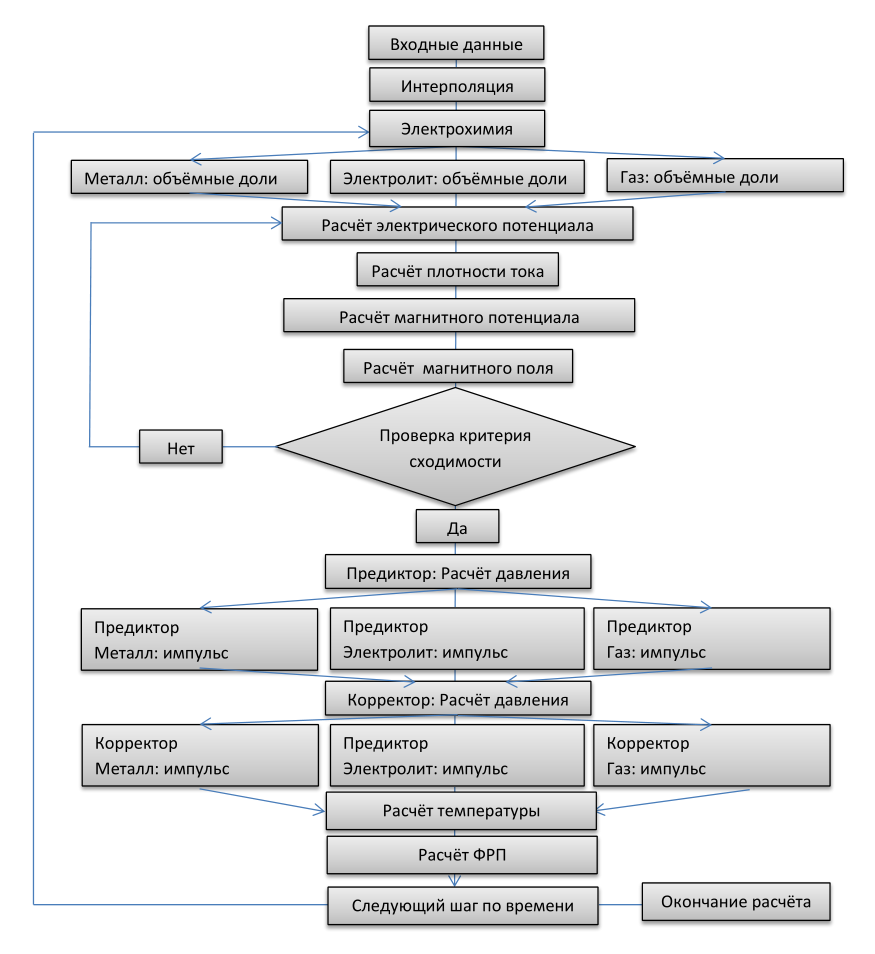
\includegraphics[width=0.8\linewidth]{scheme.png}
\caption[]{}
\label{fig:ASUTPscheme}
Схема работы АСУТП.
\end{figure}

В настоящей работе проводится математическое моделирование выхода по току конкретной алюминиевой ванны, физико-химические процессы в которой рассчитываются с помощью математической модели промышленной электролизной ванны, подробно описанной в работе~\cite{litlink:kalmykov}.

\section{Исследование способов вычисления выхода по току}

\subsection{Вычисление выхода по току по эмпирической формуле}
%\addcontentsline{toc}{section}{Вычисление выхода по току по эмпирической формуле}
Требуется провести вычисления выхода потоку при помощи эмпирической формулы (\ref{eq1}).

Приведем конкретные значения параметров в формуле (\ref{eq1}):
\begin{itemize}
\item Сила тока $I=250 $кА,
\item Длинна ванны $a=9.4$м,
\item Ширина ванны $b=3.4$м,
\item МПР 23.1 см,
\item $970 C^{\circ}$.
\end{itemize}
Таким образом плотность тока рассчитывается по формуле
\begin{equation}
i_a = \frac{I}{a \cdot b}
\end{equation}
Тогда выход потоку по формуле (\ref{eq1})
\begin{equation}
\eta=(1-2567 \cdot \frac{15.876^{0,21}}{0.688^{0.58} \cdot 0.231 \cdot e^{\frac{12940}{970}}}) \cdot 100 \approx 96.0318.
\end{equation}

Ниже на рисунках \ref{fig:SPlot}-\ref{fig:TPlot} демонстрируется вычисленная по формуле (\ref{eq1}) зависимость выхода по току от:
\begin{enumerate}
\item площади ванны при постоянной плотности тока (рис. \ref{fig:SPlot}),
\item площади ванны при постоянной силе тока (рис. \ref{fig:SaPlot}),
\item силы тока (рис. \ref{fig:IPlot}),
\item плотности тока (рис. \ref{fig:iPlot}),
\item МПР (рис. \ref{fig:LPlot}),
\item температуры расплава (рис. \ref{fig:TPlot}).
\end{enumerate}
\begin{figure}[H]
\centering
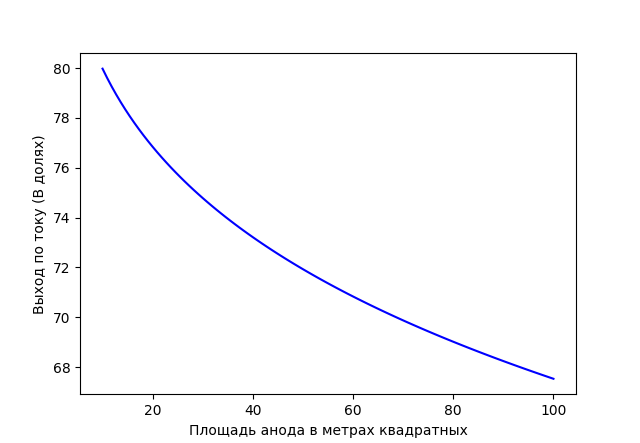
\includegraphics[width=0.8\linewidth]{S.png}
\caption{}
\label{fig:SPlot}
Зависимость выхода по току от площади ванны при постоянной плотности тока
\end{figure}

\begin{figure}[H]
\centering
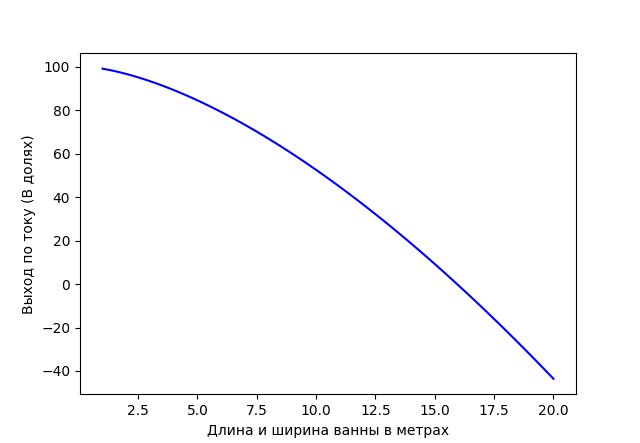
\includegraphics[width=0.8\linewidth]{Sa.png}
\caption{}
\label{fig:SaPlot}
Зависимость выхода по току от площади ванны при постоянной силе тока
\end{figure}

\begin{figure}[H]
\centering
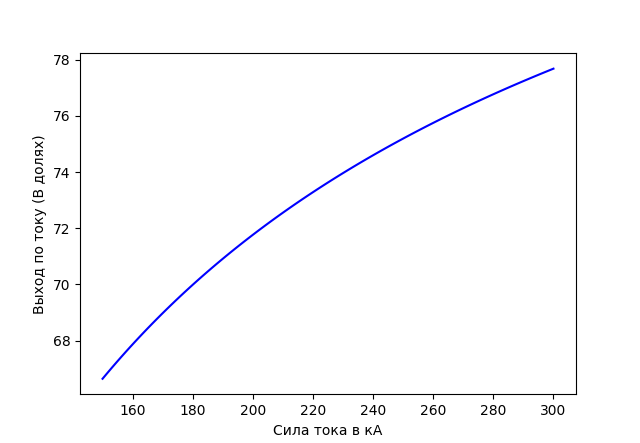
\includegraphics[width=0.8\linewidth]{I.png}
\caption{}
Зависимость выхода по току от силы тока
\label{fig:IPlot}
\end{figure}

\begin{figure}[H]
\centering
\includegraphics[width=0.8\linewidth]{i.png}
\caption{}
\label{fig:iPlot}
Зависимость выхода по току от плотности тока
\end{figure}

\begin{figure}[H]
\centering
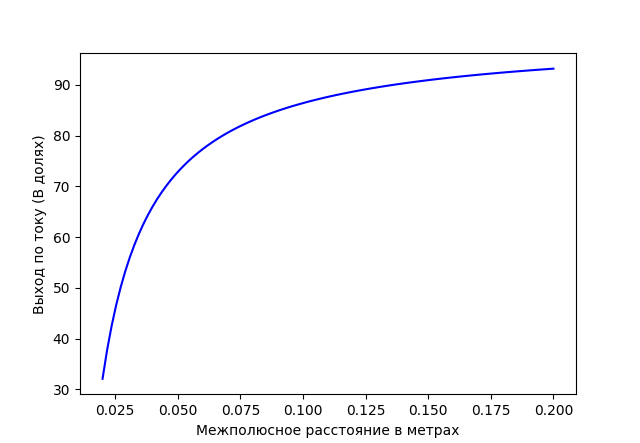
\includegraphics[width=0.8\linewidth]{L.png}
\caption{}
\label{fig:LPlot}
Зависимость выхода по току от МПР
\end{figure}

\begin{figure}[H]
\centering
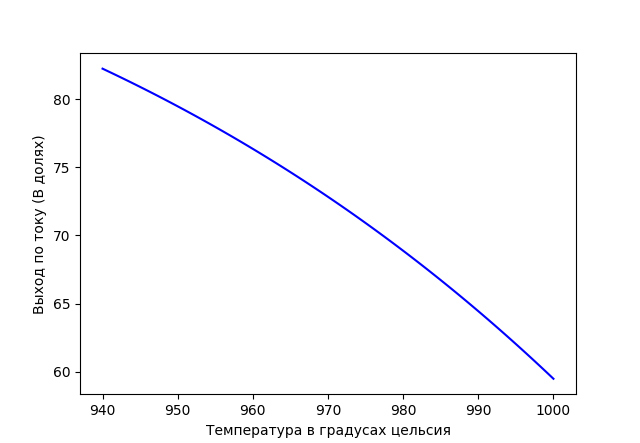
\includegraphics[width=0.8\linewidth]{T.png}
\caption{}
\label{fig:TPlot}
Зависимость выхода по току от температуры
\end{figure}

Таким образом из рисунков \ref{eq1} - \ref{eq2} видно, что управляющий параметр сильно зависит от размеров ванны и размера анода, от силы и плотности тока, от температуры и МПР. Заметим, что наиболее сложно из всех перечисленных величин замерить значение МПР. Замеры МПР на практике осуществляется путем анализа расплава металлического стержня опущенного в рабочее пространство ванны. Даже если такой эксперементальный замер производится в нескольких точках ванны, представление о минимальном МПР получается весьма приближенным, что как видно из рисунка \ref{fig:LPlot} может сильно повлиять на величину управляющего параметра выхода по току.

\subsection{Расчёт потери по току по теоретической формуле.}\label{sec:teor}

Предлагается два варианта численных методов для вычисления поверхностного интеграла в формуле (\ref{eq1}).

Используем квадратурную формулу трапеций для вычисления интеграла
\begin{equation} \label{eq:int}
I = \iint\limits_Z f(x,y) dS.
\end{equation}

Величина I по методу центральных прямоугольников на равномерной сетке по каждому направлению с шагами $h_x$ и $h_y$ с числом узлов (n+1) и (k+1) соответственно вычисляется по формуле
\begin{align}\label{eq:squaremethod}
I_{nk} = \sum\limits_{j=0}^{k} \sum\limits_{i=0}^{n} f(\frac{x_i+x_{i+1}}{2},\frac{y_j+y_{j+1}}{2}) \cdot h_x \cdot h_y
\end{align}
Ниже демонстрируется применение формулы (\ref{eq:int}) для поверхности Z(x,y) заданной в явном виде в аналитической форме. Тогда известно~\cite{ litlink:Kudryavcev}, что % chktex 36
\begin{align}
\iint\limits_Z f(x,y) dS = \label{eq:analit}
\iint\limits f(x,y) \cdot \sqrt{(1+(\frac{dZ(x,y)}{dx})^2+ (\frac{dZ(x,y)}{dy})^2)}dxdy,
\end{align}

\subsubsection*{Пример 1}\label{ex1m}
\addcontentsline{toc}{subsubsection}{Пример 1} 
Пусть поверхность раздела сред металл-электролит задана уравнением
\begin{equation} \label{eq:surf1}
Z(x,y) = 0.44 + 0.003x + 0.004y.
\end{equation}
Поверхность Z, определенная формулой (\ref{eq:surf1}), изображена на рисунке \ref{fig:H1Surf}. Площадь анодов для этой ванны возьмем $40$.

Будем считать, что эта поверхность является разделом металл - электролит электролизной ванны размеры которой зафиксированы выше. Тогда величина l соответствует минимальному расстоянию от поверхности Z до подошвы анода, $l=1 cm$.

\begin{figure}[H]
\centering
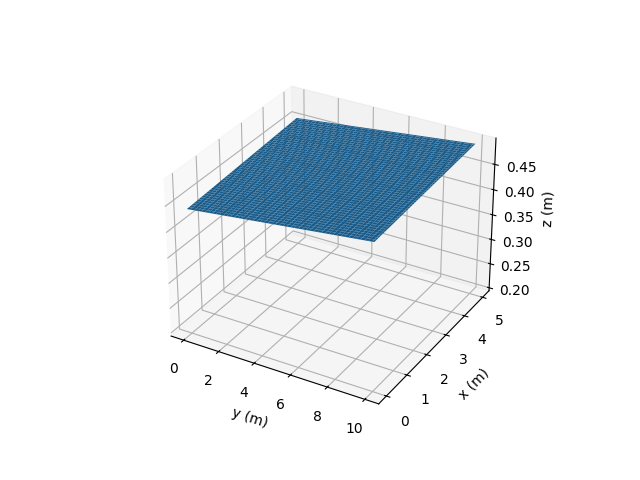
\includegraphics[width=0.8\linewidth]{First_surface.png}
\caption{}
\label{fig:H1Surf}
Разделяющая поверхность
\end{figure}

Проведем вычисления потери выхода по току по формуле (\ref{eq2}). При этом интеграл по поверхности будем вычислять по формуле (\ref{eq:analit}).


Аналитическое вычисление по формуле (\ref{eq:analit})
\begin{align} \label{eq:analit1:min}
\Delta \eta = 0,1 \cdot \frac{0.01}{40} \int\limits_0^{10} \int\limits_0^5 \frac{\sqrt{1+(0,003)^2+(0,004)^2}}{0.44 + 0.003x + 0.004y} dy dx = \notag \\
= \frac{0,1 \cdot 0.01\sqrt{1+(0,003)^2+(0,004)^2}}{40 \cdot 0,004} \cdot \notag \\
\cdot \int\limits_0^{10} \ln(0.44 + 0.003x + 0.004y)|_0^5 dx = \notag \\
= \frac{0,1 \cdot 0.01\sqrt{1+(0,003)^2+(0,004)^2}}{40 \cdot 0,004} \cdot \notag \\
\cdot \bigl(\int\limits_0^{10} \ln(0.44 + 0.003x + 0.02)dx - \int\limits_0^{10} \ln(0.44 + 0.003x)dx \bigr) = \notag \\
= \frac{-0,1 \cdot 0.01\sqrt{1+(0,003)^2+(0,004)^2}}{40 \cdot 0,004 \cdot 0.003} \cdot \notag \\
\cdot \bigl(((0,46+0,003x) \cdot \ln(0,46+0,003x) - (0,46+0,003x))|_0^{10} - \notag \\
- ((0,46+0,003x) \cdot \ln(0,346+0,003x) - (0,346+0,003x))|_0^{10}\bigr) = \notag \\
= \frac{-0,1 \cdot 0.01\sqrt{1+(0,003)^2+(0,004)^2}}{40 \cdot 0,004 \cdot 0.003} \cdot \notag \\
\cdot \bigl(0,47 \ln(0.47)-0,44 \ln(0,44)-0,03- \notag \\
- (0,49 \ln(0,49)-0,46 \ln(0,46)-0,03)\bigr) = \notag \\
= 0.002689559
\end{align}
Вычисления по квадратурной формуле (\ref{eq:squaremethod}), n=k=100
\begin{align}\label{eq:sq1min10}
\Delta \eta = 0,1 \cdot \frac{0.01}{50.000625} \int\limits_0^{10} \int\limits_0^5 \frac{\sqrt{1+(0,003)^2+(0,004)^2}}{0.44 + 0.003x + 0.004y} dy dx \approx \notag \\ \approx 0.0026910167819670706
\end{align}
Вычисления по квадратурной формуле (\ref{eq:squaremethod}), n=k=50
\begin{align}\label{eq:sq1min5}
\Delta \eta = 0,1 \cdot \frac{0.01}{50.000625} \int\limits_0^{10} \int\limits_0^5 \frac{\sqrt{1+(0,003)^2+(0,004)^2}}{0.44 + 0.003x + 0.004y} dy dx \approx \notag \\ \approx 0.002692510716716919
\end{align}

Проведем аналогичные вычисления для другого значения l, пусть $l=0.06$ (соответствует точке на поверхности Z(x,y) в центре). % chktex 36

Аналитическое решение по формуле (\ref{eq:analit})
\begin{align} \label{eq:analit1:med}
\Delta \eta = 0,1 \cdot \frac{0.01}{40} \int\limits_0^{10} \int\limits_0^5 \frac{\sqrt{1+(0,003)^2+(0,004)^2}}{0.44 + 0.003x + 0.004y} dy dx = \notag \\
= \frac{0,1 \cdot 0.01\sqrt{1+(0,003)^2+(0,004)^2}}{40 \cdot 0,004} \cdot \notag \\
\cdot \int\limits_0^{10} \ln(0.44 + 0.003x + 0.004y)|_0^5 dx = \notag \\
= \frac{0,1 \cdot 0.01\sqrt{1+(0,003)^2+(0,004)^2}}{40 \cdot 0,004} \cdot \notag \\
\cdot \bigl(\int\limits_0^{10} \ln(0.44 + 0.003x + 0.02)dx - \int\limits_0^{10} \ln(0.44 + 0.003x)dx \bigr) = \notag \\
= \frac{-0,1 \cdot 0.01\sqrt{1+(0,003)^2+(0,004)^2}}{40 \cdot 0,004 \cdot 0.003} \cdot \notag \\
\cdot \bigl(((0,46+0,003x) \cdot \ln(0,46+0,003x) - (0,46+0,003x))|_0^{10} - \notag \\
- ((0,46+0,003x) \cdot \ln(0,346+0,003x) - (0,346+0,003x))|_0^{10}\bigr) = \notag \\
= \frac{-0,1 \cdot 0.01\sqrt{1+(0,003)^2+(0,004)^2}}{40 \cdot 0,004 \cdot 0.003} \cdot \notag \\
\cdot \bigl(0,47 \ln(0.47)-0,44 \ln(0,44)-0,03- \notag \\
- (0,49 \ln(0,49)-0,46 \ln(0,46)-0,03)\bigr) = \notag \\
= 0.016137327
\end{align}
Вычисления по квадратурной формуле (\ref{eq:squaremethod}), n=k=100
\begin{align}\label{eq:sq1med10}
0,1 \cdot \frac{0.06}{40} \int\limits_0^{10} \int\limits_0^5 \frac{\sqrt{1+(0,003)^2+(0,004)^2}}{0.44 + 0.003x + 0.004y} dy dx \approx \notag \\ \approx 0.016146100691802452
\end{align}
Вычисления по квадратурной формуле (\ref{eq:squaremethod}), n=k=50
\begin{align}\label{eq:sq1med5}
0,1 \cdot \frac{0.06}{40} \int\limits_0^{10} \int\limits_0^5 \frac{\sqrt{1+(0,003)^2+(0,004)^2}}{0.44 + 0.003x + 0.004y} dy dx \approx \notag \\ \approx 0.01615506430030167
\end{align}

Проведем вычисления для $l=0.11$ (соответствует точке на поверхности Z(x,y) в правом верхнем углу). % chktex 36

Аналитическое решение по формуле (\ref{eq:analit})
\begin{align}\label{eq:analit1:max}
\Delta \eta = 0,1 \cdot \frac{0.11}{40} \int\limits_0^{10} \int\limits_0^5 \frac{\sqrt{1+(0,003)^2+(0,004)^2}}{0.44 + 0.003x + 0.004y} dy dx = \notag \\
= \frac{0,1 \cdot 0.01\sqrt{1+(0,003)^2+(0,004)^2}}{40 \cdot 0,004} \cdot \notag \\
\cdot \int\limits_0^{10} \ln(0.44 + 0.003x + 0.004y)|_0^5 dx = \notag \\
= \frac{0,1 \cdot 0.01\sqrt{1+(0,003)^2+(0,004)^2}}{40 \cdot 0,004} \cdot \notag \\
\cdot \bigl(\int\limits_0^{10} \ln(0.44 + 0.003x + 0.02)dx - \int\limits_0^{10} \ln(0.44 + 0.003x)dx \bigr) = \notag \\
= \frac{-0,1 \cdot 0.01\sqrt{1+(0,003)^2+(0,004)^2}}{40 \cdot 0,004 \cdot 0.003} \cdot \notag \\
\cdot \bigl(((0,46+0,003x) \cdot \ln(0,46+0,003x) - (0,46+0,003x))|_0^{10} - \notag \\
- ((0,46+0,003x) \cdot \ln(0,346+0,003x) - (0,346+0,003x))|_0^{10}\bigr) = \notag \\
= \frac{-0,1 \cdot 0.01\sqrt{1+(0,003)^2+(0,004)^2}}{40 \cdot 0,004 \cdot 0.003} \cdot \notag \\
\cdot \bigl(0,47 \ln(0.47)-0,44 \ln(0,44)-0,03- \notag \\
- (0,49 \ln(0,49)-0,46 \ln(0,46)-0,03)\bigr) = \notag \\
= 0.02958512
\end{align}
Вычисления по квадратурной формуле (\ref{eq:squaremethod}), n=k=100
\begin{align}\label{eq:sq1max10}
\Delta \eta = (1- \eta_0) \cdot \frac{l}{S} \cdot \iint\limits_Z \frac{\sqrt{(1+(\frac{dz}{dx})^2+ (\frac{dz}{dy})^2)}}{H(x,y)}dxdy = \notag \\
= 0,1 \cdot \frac{0.11}{40} \int\limits_0^{10} \int\limits_0^5 \frac{\sqrt{1+(0,003)^2+(0,004)^2}}{0.44 + 0.003x + 0.004y} dy dx \approx \notag \\
\approx 0.02960118460163804
\end{align}
Вычисления по квадратурной формуле (\ref{eq:squaremethod}), n=k=50
\begin{align}\label{eq:sq1max5}
\Delta \eta = (1- \eta_0) \cdot \frac{l}{S} \cdot \iint\limits_Z \frac{\sqrt{(1+(\frac{dz}{dx})^2+ (\frac{dz}{dy})^2)}}{H(x,y)}dxdy = \notag \\
= 0,1 \cdot \frac{0.2}{40} \int\limits_0^{10} \int\limits_0^5 \frac{\sqrt{1+(0,003)^2+(0,004)^2}}{0.44 + 0.003x + 0.004y} dy dx \approx \notag \\ 
\approx 0.029617617883886373
\end{align}

Анализ результатов проведенных расчетов показывает, что величина l сильно влияет на значение параметра потери выхода по току. При этом расчеты вариантов b наиболее близки к соответствующим значениям, вычисленным аналитически. 

\subsubsection*{Пример 2}\label{ex2m}
\addcontentsline{toc}{subsubsection}{Пример 2}
Пусть поверхность раздела сред металл-электролит задана уравнением
\begin{equation}\label{eq:surf2}
z(x,y)=0,44+0,05 \cdot \sin(x) \cdot \cos(y)
\end{equation}

Поверхность Z, определенная формулой (\ref{eq:surf2}), изображена на рисунке \ref{fig:H2Surf}. Площадь андов для этой ванны будем считать $40 m^2$.

Будем считать, что эта поверхность является разделом металл - электролит электролизной ванны размеры которой зафиксированы выше. Тогда величина l соответствует минимальному расстоянию от поверхности Z до подошвы анода, $l=1 cm$.

\begin{figure}[H]
\centering
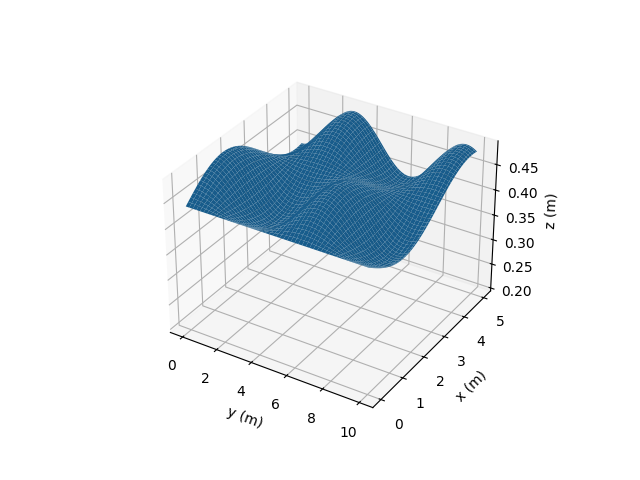
\includegraphics[width=0.8\linewidth]{Second_surface.png}
\caption{}
\label{fig:H2Surf}
Разделяющая поверхность
\end{figure}


Вычисления по квадратурной формуле (\ref{eq:squaremethod}), n=k=100
\begin{align}\label{eq:sq2min10}
\Delta \eta = 0,1 \cdot \frac{0,01}{40} \cdot \notag \\
\cdot \int\limits_0^{10} \int\limits_0^5 \frac{\sqrt{1+0.05 \cos(x)\cos(y)-0.05 \sin(x)\sin(y)}}{0.44 + 0.05 \sin(x)\cos(y)} dy dx \approx \notag \\ \approx 0.0028705181744004275
\end{align}
Вычисления по квадратурной формуле (\ref{eq:squaremethod}), n=k=50
\begin{align}\label{eq:sq2min5}
\Delta \eta = 0,1 \cdot \frac{0,05}{40}  \cdot \notag \\
\cdot \int\limits_0^{10} \int\limits_0^5 \frac{\sqrt{1+0.05 \cos(x)\cos(y)-0.05 \sin(x)\sin(y)}}{0.44 + 0.05 \cdot \sin(x) \cdot \cos(y)} dy dx \approx \notag \\ \approx 0.002870213860349491
\end{align}

Проведем аналогичные вычисления для другого значения l, пусть $l=0.06$ (соответствует точке на поверхности Z(x,y) в точках $\sin(x)=0$ или $\cos(y)=0$). %chktex 36

Вычисления по квадратурной формуле (\ref{eq:squaremethod}), n=k=100
\begin{align}\label{eq:sq2med10}
\Delta \eta = 0,1 \cdot \frac{0,06}{40} \cdot \notag \\
\cdot \int\limits_0^{10} \int\limits_0^5 \frac{\sqrt{1+0.05 \cos(x)\cos(y)-0.05 \sin(x)\sin(y)}}{0.44 + 0.05 \cdot \sin(x) \cdot \cos(y)} dy dx \approx \notag \\ \approx 0.01722310904640258
\end{align}
Вычисления по квадратурной формуле (\ref{eq:squaremethod}), n=k=50
\begin{align}\label{eq:sq2med5}
\Delta \eta = 0,1 \cdot \frac{0,06}{40} \cdot \notag \\
\cdot \int\limits_0^{10} \int\limits_0^5 \frac{\sqrt{1+0.05 \cos(x)\cos(y)-0.05 \sin(x)\sin(y)}}{0.44 + 0.05 \cdot \sin(x) \cdot \cos(y)} dy dx \approx \notag \\ \approx 0.017221283162096944
\end{align}

Проведем вычисления для $l=0.11$ (соответствует точке на поверхности Z(x,y) на 'пике'). %chktex 36

Аналитическое решение по формуле (\ref{eq:analit})

Вычисления по квадратурной формуле (\ref{eq:squaremethod}), n=k=100
\begin{align}\label{eq:sq2max10}
\Delta \eta = 0,1 \cdot \frac{0.11}{40} \cdot \notag \\
\cdot \int\limits_0^{10} \int\limits_0^5 \frac{\sqrt{1+0.05 \cos(x)\cos(y)-0.05 \sin(x)\sin(y)}}{0.44 + 0.05 \cdot \sin(x) \cdot \cos(y)} dy dx \approx \notag \\ \approx 0.0315756999184048
\end{align}
Вычисления по квадратурной формуле (\ref{eq:squaremethod}), n=k=50
\begin{align}\label{eq:sq2max5}
\Delta \eta = 0,1 \cdot \frac{0.11}{40} \cdot \notag \\
\cdot \int\limits_0^{10} \int\limits_0^5 \frac{\sqrt{1+0.05 \cos(x)\cos(y)-0.05 \sin(x)\sin(y)}}{0.44 + 0.05 \cdot \sin(x) \cdot \cos(y)} dy dx \approx \notag \\ \approx 0.03157235246384434
\end{align}

\subsection{Модифицированная теоретическая формула вычисления потери по току.}\label{sec:mod}

Для расчета потери выхода по току по теоретической формуле (\ref{eq2}) используется параметр выхода по току при плоской границе раздела сред $\eta_0$. Поскольку поверхность раздела сред Z меняется во времени, то ее площадь S также меняется во времени. В свою очередь, величина l может быть разной в зависимости от точки, в которой проводится измерение. Как показано в работе~\cite{litlink:kalmykov}, граница раздела сред электролит-газ, соответствующая зоне обратного окисления металла, также сильно влияет на величину l, а значит, на величину потерь выхода по току.

В формуле (\ref{eq2}) значения параметров l и S являются константами, которые определяются опытным путем с большой погрешностью. Поэтому в настоящей работе предлагается следующая модификация формулы (\ref{eq2}).
\begin{equation} \label{eq:modeq2}
\Delta \eta = (1- \eta_0) \cdot \frac{1}{S} \cdot \iint\limits_Z \frac{l(x,y)}{H(x,y)}dS.
\end{equation}

Ниже приводится вычисление тремя способами значения потери по току для различных поверхностей Z(x,y).	% chktex 36

\subsubsection*{Пример 1}
\addcontentsline{toc}{subsubsection}{Пример 1}

Поверхность Z, определенная формулой (\ref{eq:surf1}), изображена на рисунке \ref{fig:H1Surf}. Площадь анодов равняется $40$ также, как и выше.

Вычисления по квадратурной формуле (\ref{eq:squaremethod}), n=k=100
\begin{align}
\Delta \eta = 0,1 \cdot \frac{1}{40} \int\limits_0^{10} \int\limits_0^5 (0.06 - 0.44 + 0.003x + 0.004y) \cdot \notag \\
\cdot \sqrt{1+(0,003)^2+(0,004)^2}/ \notag \\ 
/(0.44 + 0.003x + 0.004y) dy dx \approx \notag \\ \approx 0.009549276608118927
\end{align}
Вычисления по квадратурной формуле (\ref{eq:squaremethod}), n=k=50
\begin{align}
\Delta \eta = 0,1 \cdot \frac{1}{40} \int\limits_0^{10} \int\limits_0^5 (0.06 - 0.44 + 0.003x + 0.004y) \cdot \notag \\
\cdot \sqrt{1+(0,003)^2+(0,004)^2}/ \notag \\ 
/(0.44 + 0.003x + 0.004y) dy dx \approx \notag \\ \approx 0.00962397334561231
\end{align}

\subsubsection*{Пример 2}
\addcontentsline{toc}{subsubsection}{Пример 2}

Поверхность Z, определенная формулой (\ref{eq:surf1}), изображена на рисунке \ref{fig:H1Surf}. Площадь анодов равняется $40$ также, как и выше.

Вычисления по квадратурной формуле (\ref{eq:squaremethod}), n=k=100
\begin{align}
\Delta \eta = 0,1 \cdot \frac{1}{40} \cdot \notag \\
\cdot \int\limits_0^{10} \int\limits_0^5 (0,06 - 0,05 \sin(x)\cos(y)) \cdot \notag \\
\cdot \sqrt{1+0.05 \cos(x)\cos(y)-0.05 \sin(x)\sin(y)}/ \notag \\
/(0.44 + 0.05 \sin(x)\cos(y)) dy dx \approx \notag \\ \approx 0.018253636056426627
\end{align}
Вычисления по квадратурной формуле (\ref{eq:squaremethod}), n=k=4
\begin{align}
\Delta \eta = 0,1 \cdot \frac{1}{40} \cdot \notag \\
\cdot \int\limits_0^{10} \int\limits_0^5 (0,06 - 0,05 \sin(x)\cos(y)) \cdot \notag \\
\cdot \sqrt{1+0.05\cos(x)\cos(y)-0.05\sin(x)\sin(y)}/ \notag \\
/(0.44 + 0.05\sin(x)\cos(y)) dy dx \approx \notag \\ \approx 0.018252353331560892
\end{align}

Модифицированная формула дает существенно отличный результат от полученного в формуле (\ref{eq2}).

\section{Вычисление потери выхода по току для поверхности границы раздела сред металл - электролит произвольного вида.}
\subsection{Вывод формулы вычисления поверхности при помощи метода триангуляции}

В пунктах \ref{sec:teor} и \ref{sec:mod} поверхность раздела задавалась аналитически. Однако в вычислительном комплексе математического моделирования процесса промышленного электролиза алюминия границы раздела сред металл-электролит и газ-электролит получаются в результате численного расчета и задаются таблично. Поэтому интегралы в формулах (\ref{eq1}) и (\ref{eq:modeq2}) эффективно вычислять методом триангуляции.

В работах~\cite{litlink:scvortsov} и~\cite{litlink:shirok} подробно описаны способы построения триангуляции для сложных поверхностей с неравномерно заданными на плоскости точками. В настоящей работе предлагается алгоритм вычисления поверхностного интеграла для границы раздела металл-электролит произвольной конфигурации, адаптированного к равномерной сетке по каждому пространственному направлению. При этом именно эта равномерная сетка используется в вычислениях комплекса, реализующем математическую модель электролиза алюминия в промышленной ванне (см.~\cite{litlink:kalmykov}). Однако эти методы сложны в реализации.

Выпишем формулы триангуляции для простой прямоугольной поверхности с разбиением на элементарные треугольники.

На плоскости водится равномерная сетка размером $N$ на $M$ с шагами $x_h$, $h_y$ и узлами $P_{i,j}$. В узлах этой сетки таблично задается подынтегральная функция $f_{i,j}$. Плоскость разбивается на $2 \cdot N \cdot M$ прямоугольных треугольников, как показано на рисунке \ref{fig:grid}.

\begin{figure}[H]
\centering
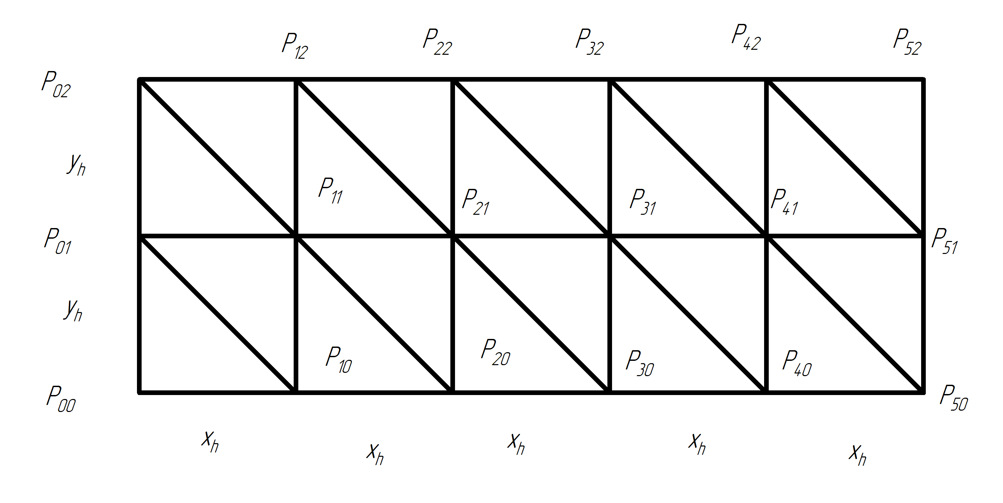
\includegraphics[width=0.8\linewidth]{Сетка.png}
\caption{}
\label{fig:grid}
Разбиение рассчетной области на треугольники.
\end{figure}

Каждый из этих треугольников соответствует поверхностному треугольнику в поверхности Z, как показано на рисунке \ref{fig:triangle}.

\begin{figure}[H]
\centering
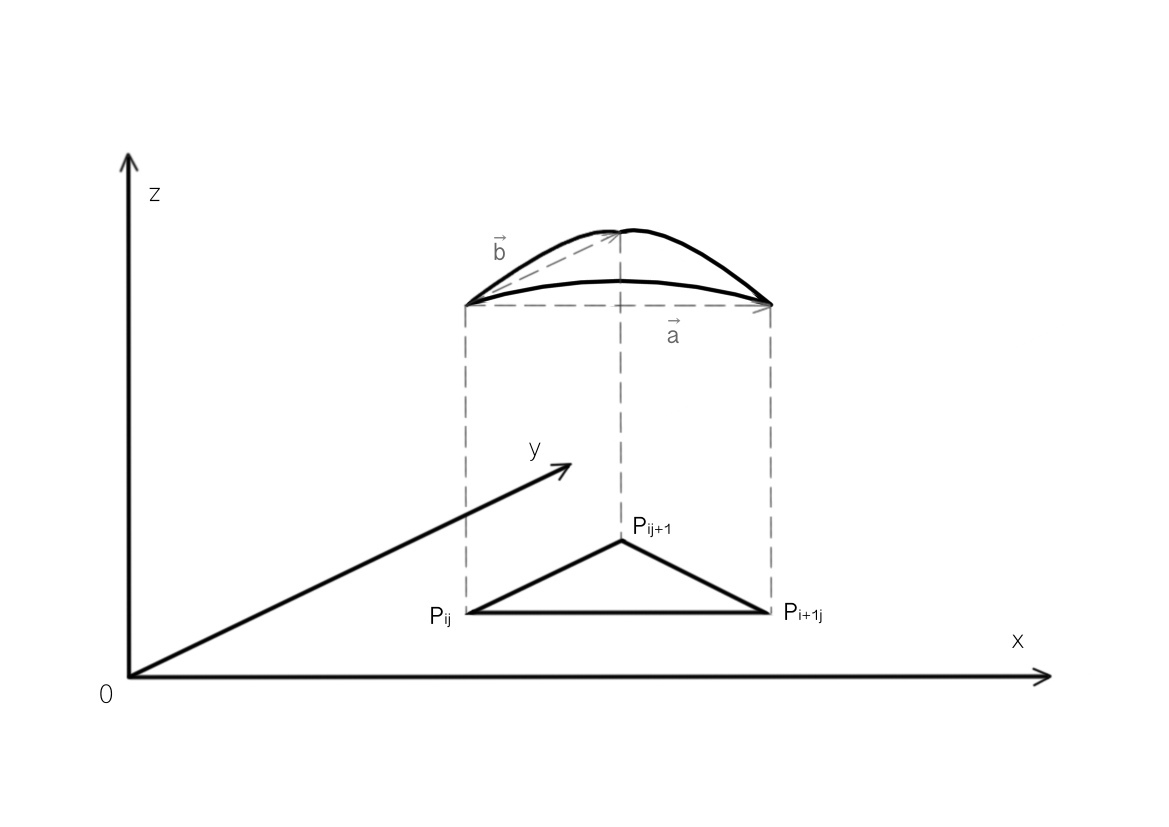
\includegraphics[width=0.8\linewidth]{Triangle.jpg}
\caption{}
\label{fig:triangle}
Проекция поверхности раздела на расчетную сетку.
\end{figure}

Площади поверхностных треугольников $P_{i,j}, P_{i,j+1}, P_{i+1,j}$ считаются по формуле 

\begin{align}\label{eq:triangle_square}
S_{\triangle_{i,j}^1} = \frac{1}{2} \lvert [\overline{P_{i,j}P_{i,j+1}};\overline{P_{i,j}P_{i+1,j}}] \rvert = \lvert \frac{1}{2} 
\begin{vmatrix}
  I & J & K \\
  h_x & 0 & f_{i+1,j}-f_{i,j} \\
  0 & h_y & f_{i,j+1}-f_{i,j}
\end{vmatrix}
\rvert
= \notag \\
= \lvert I \cdot (-(f_{i+1,j}-f_{i,j}) \cdot h_y) - h_x \cdot (J \cdot (f_{i,j+1}-f_{i,j}) - h_y \cdot K) \rvert = \notag \\
= \lvert I \cdot h_y \cdot f_{i,j} -I \cdot h_y \cdot f_{i+1,j} - h_x \cdot J \cdot f_{i,j+1}+ h_x \cdot J \cdot f_{i,j} + h_x \cdot h_y \cdot K \rvert = \notag \\
= (h_y \cdot f_{i,j} - \cdot h_y \cdot f_{i+1,j})^2 + (h_x \cdot f_{i,j} - h_x \cdot f_{i,j+1})^2 + (h_x \cdot h_y)^2 \\
S_{\triangle_{i,j}^2} = \frac{1}{2} \lvert [\overline{P_{i+1,j+1}P_{i,j+1}};\overline{P_{i+1,j+1}P_{i+1,j}}] \rvert = \notag \\
= (h_y \cdot f_{i+1,j+1} - \cdot h_y \cdot f_{i+1,j})^2 + (h_x \cdot f_{i+1,j+1} - h_x \cdot f_{i,j+1})^2 + (h_x \cdot h_y)^2,
\end{align}
где I,J,K орты соответственно осей X,Y,Z.

Пронумеруем треугольники, как показано на рисунке \ref{fig:triangle_numeration}.

\begin{figure}[H]
\centering
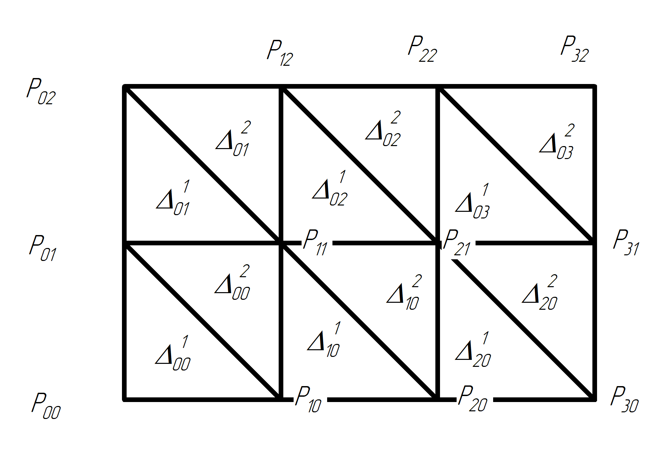
\includegraphics[width=0.8\linewidth]{triangle_numeration.png}
\caption{}
\label{fig:triangle_numeration}
Порядок нумерации введённых треугольников на расчётной сетке.
\end{figure}

Каждому $\triangle^n_{i,j}$ соответствует значение функции $F^n_{i,j}$, получим значение для двумерного по аналогии с одномерным случаем:

\begin{enumerate}
\item Одномерный случай.

В одномерном случае рассматривается интеграл
\begin{align}
I= \int\limits_a^b f(x) dx.
\end{align}
Для его вычисления область интегрирования (отрезок $[a,b]$) разбивается на элементарные отрезки $[x_i, x_{i+1}]$. Каждому элементарному отрезку соответствует значение функции $f_i$, тогда приближенное значение интеграла на этом отрезке $\widetilde{I}=(x_{i+1}-x_{i}) \cdot f_i$.

Построим интерполяционный полином Лагранжа на этом отрезке
\begin{align}
L(x) = \frac{x-x_{i+1}}{x_i-x_{i+1}} \cdot f_i+ \frac{x-x_i}{x_{i+1}-x_{i}} \cdot f_{i+1} = \notag \\
= \frac{1}{x_{i+1}-x_{i}} ((x-x_{i})\cdot f_{i+1}-(x-x_{i+1}) \cdot f_{i}).
\end{align}
Тогда,
\begin{align}
\widetilde{I} = \int\limits_{x_{i}}^{x_{i+1}} L(x) dx = \notag \\
= \frac{1}{x_{i+1}-x_{i}} (f_{i+1} \int\limits_{x_{i}}^{x_{i+1}} (x-x_{i}) dx - f_i \int\limits_{x_{i}}^{x_{i+1}} (x-x_{i+1}) dx) = \notag \\
= \frac{1}{x_{i+1}-x_{i}} (f_{i+1} \cdot (\frac{1}{2} (x_{i+1}^2 - x_{i}^2) -x_i x_{i+1}+x_{i}^2)) - \notag \\
- f(x_{i}) (\frac{1}{2} (x_{i+1}^2-x_{i}^2)-x_{i+1}^2+x_i x_{i+1}) = \notag \\
= \frac{1}{x_{i+1}-x_{i}} \cdot \notag \\
\cdot (f_{i+1} \cdot (\frac{1}{2} (x_{i+1}^2 + x_{i}^2) -x_i x_{i+1}) + f_i (\frac{1}{2}(x_{i+1}^2+x_{i}^2)-x_i x_{i+1})) = \notag \\
= \frac{1}{x_{i+1}-x_{i}} (f_{i+1}+ f_i) \cdot (\frac{1}{2} (x_{i+1}^2 + x_{i}^2) -x_i x_{i+1}) = \notag \\
= (x_{i+1}-x_{i}) \cdot \frac{1}{2}(f_i+f_{i+1})
\end{align}

Тогда f на элементарном отрезке.
\begin{align}
F_i = \frac{1}{2}(f_{i}+f_{i+1})
\end{align}

$F_i$ аппроксимирует значение функции со вторым порядком точности~\cite{litlink:samarskiy} в середине отрезка.

Аналогично с одномерным случаем вычислим значение двумерного поверхностного интеграла.

\item Двумерный случай

Применим вышеописанный метод разбиения поверхности. Разобьём поверхность на элементарные фрагменты, как показано на рисунке 1. Каждому из которых поставим в соответствие треугольник ABC.

\begin{figure}[H]
\centering
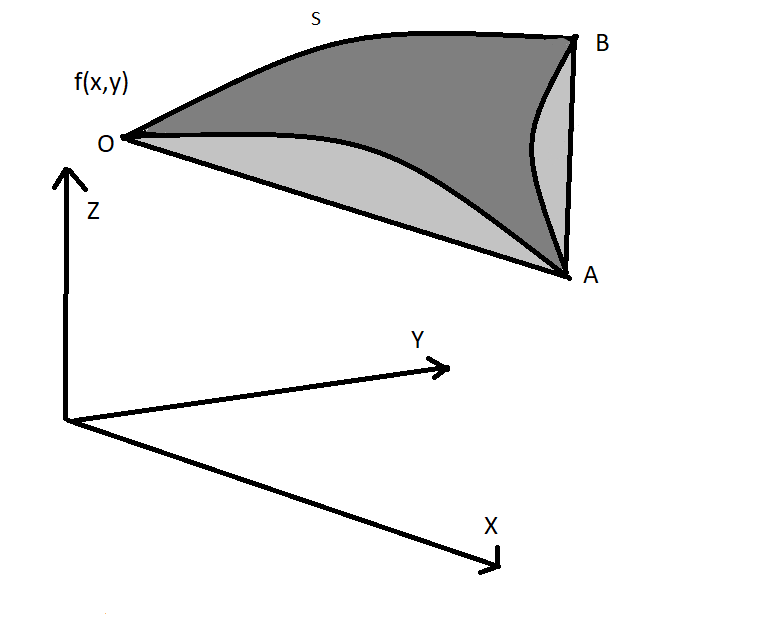
\includegraphics[width=0.8\linewidth]{triangleL.png}
\caption[]{}
\label{fig:L}
Фрагмент поверхности с соответствующим ему элементарным треугольником.
\end{figure}

\begin{figure}[H]
\centering
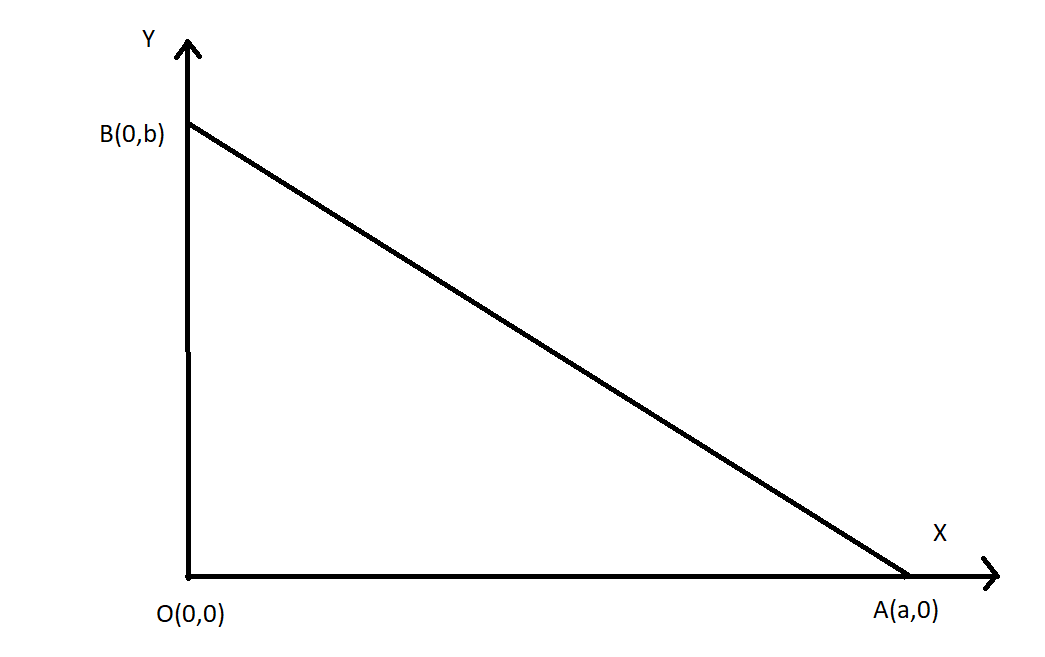
\includegraphics[width=0.8\linewidth]{triangleOAB.png}
\caption[]{}
\label{fig:ABC}
Локализация треугольника OAB.
\end{figure}

Ниже приводится уравнение плоскости, которому принадлежит треугольник OAB, в каноническом виде.
\begin{align}
\begin{vmatrix}\label{eq:surfeq}
  x-0	& y-0	& z-f(O)	\\
  a		& 0		& f(A)-f(O)	\\
  0		& b		& f(B)-f(O)
\end{vmatrix}
= 0
\end{align}
Выразим координату $z$ из уравнения (\ref{eq:surfeq}).
\begin{align}
z = xb(f(A)-f(O))-(ya(f(B)+f(O))+abf(O)) \div ab = \notag \\
= \frac{x}{a}(f(A)-f(O))+\frac{y}{b}(f(B)-f(O)) + f(O) \label{eq:z} \\
L_1 = \frac{x}{a}(f(A)-f(O)) \\
L_2 = \frac{y}{b}(f(B)-f(O))
\end{align}
Подставим выражение (\ref{eq:z}) в интеграл $\widetilde{I}$. Получим:
\begin{align}
\widetilde{I} = \iint\limits_{\triangle} L_1 dx dy+\iint\limits_{\triangle} L_2 dx dy+\iint\limits_{\triangle} f(O)= \notag \\
= \int\limits_0^a dx \int\limits_0^{b-x \frac{b}{a}} L_1 dy + \int\limits_0^b dy \int\limits_0^{a-y \frac{a}{b}} L_2 dx + ab f(O)- \frac{ab}{2}f(O) = \notag \\
= \int\limits_0^a L_1 (b-x \frac{b}{a}) dx + \int\limits_0^b L_2 (a-y \frac{a}{b}) dy + \frac{ab}{2} f(O) = \notag \\
= \int\limits_0^a \frac{x}{a} (f(A)-f(O)) (b-x \frac{b}{a}) dx + \notag \\
+ \int\limits_0^b \frac{y}{b} (f(B)-f(O)) (a-y \frac{a}{b}) dy + \frac{ab}{2} f(O) = \notag
\end{align}

\begin{align}
= \int\limits_0^a x \frac{b}{a} (f(A)-f(O)) dx - \int\limits_0^a x^2 \frac{b}{a^2} (f(A)-f(O)) dx + \notag \\
+ \int\limits_0^b y \frac{a}{b} (f(B)-f(O)) dy - \int\limits_0^b y^2 \frac{a}{b^2}(f(B)-f(O))dy + \frac{ab}{2} f(O) = \notag \\
= \frac{ab}{2} (f(A)-f(O)) - \frac{ab}{3} (f(B)-f(O)) + \notag \\
+ \frac{ab}{2}(f(B)-f(O)) - \frac{ab}{3} (f(B)-f(O)) + \frac{ab}{2} f(O) = \notag \\
= \frac{ab}{6} (f(A)-f(O)) + \frac{ab}{6} (f(B)-f(O)) + \frac{ab}{2} f(O) = \notag \\
= \frac{ab}{6} (f(A)+f(B)-2f(0)) + \frac{ab}{2} f(O) = \notag\\
= \frac{ab}{6} (f(A)+f(B)+f(0)) = \notag \\
= \frac{ab}{2} \cdot \frac{1}{3}(f(A)+f(O)+f(B)) = \widetilde{I}\label{eq:trifunc}
\end{align}

Таким образом, из выражения (\ref{eq:trifunc}) следует, что треугольнику OAB соответствует значение функции F, которая вычисляется по формуле:

\begin{equation}
F =  \frac{1}{3}(f(A)+f(O)+f(B))
\end{equation}

\end{enumerate}

Таким образом, элементарному треугольнику $\triangle_{i,j}$ естественно поставить в соответствие формулы (\ref{eq:f1}) и (\ref{eq:f2}).

\begin{align}
F^1_{i,j} = \frac{1}{3}(f_{i,j}+f_{i,j+1}+f_{i+1,j}), \label{eq:f1}\\
F^2_{i,j} = \frac{1}{3}(f_{i+1,j+1}+f_{i,j+1}+f_{i+1,j}). \label{eq:f2}
\end{align}

Следовательно, поверхностный интеграл (\ref{eq:int}) будем вычислять по следующей формуле
\begin{align}\label{eq:trint}
I \approx \sum_{i=0}^{N-1} \sum_{j=0}^{M-1} I_{i,j} = \sum_{i=0}^{N-1} \sum_{j=0}^{M-1} (S_{\triangle_{i,j}^1} \cdot F_{i,j}^1 + S_{\triangle_{i,j}^2} \cdot F_{i,j}^2) = \notag \\
= \sum_{i=0}^{N-1} \sum_{j=0}^{M-1} ((h_y \cdot f_{i,j} - h_y \cdot f_{i+1,j})^2 + (h_x \cdot f_{i,j} - h_x \cdot f_{i,j+1})^2 + (h_x \cdot h_y)^2 + \notag \\
+ \frac{1}{3}(f_{i,j}+f_{i,j+1}+f_{i+1,j}) + \notag \\
+(h_y \cdot f_{i+1,j+1} - h_y \cdot f_{i+1,j})^2 + (h_x \cdot f_{i+1,j+1} - h_x \cdot f_{i,j+1})^2 + (h_x \cdot h_y)^2 + \notag \\
+\frac{1}{3}(f_{i+1,j+1}+f_{i,j+1}+f_{i+1,j}))
\end{align}

Тогда значения потерь выхода по току по эмпирическим формулам (\ref{eq2}) и (\ref{eq:trint}) приближенно вычисляются следующим образом.



\subsection{Исследование точности разработанного метода}

Для оценки полученного выше метода воспользуемся правилом Рунге~\cite{litlink:samarskiy}:

\begin{equation}\label{eq:runge1}
|I-I_{\frac{h}{2}}| \approx \frac{|I_{\frac{h}{2}}-I_{h}|}{2^m-1}
\end{equation}
где $I_h$ значение, полученное исследуемым методом при шаге сетки $h$, $I_{\frac{h}{2}}$ значение, полученное исследуемым методом при шаге сетки $\frac{h}{2}$ $I$ - точное значение интеграла, $m$ - порядок точности исследуемого метода.

Исследуем порядок точности приведенного выше метода вычисления поверхностного интеграла на двух примерах, имеющих аналитическое решение.

\subsubsection*{Тест 1}

Рассмотрим поверхность z(x,y) (\ref{eq:surfcyl}) %chktex 36
\begin{equation}\label{eq:surfcyl}
z(x,y) = \sqrt{4-(x-1)^2}, x \in [0,2], y \in [0,5].
\end{equation}

\begin{figure}[H]
\centering
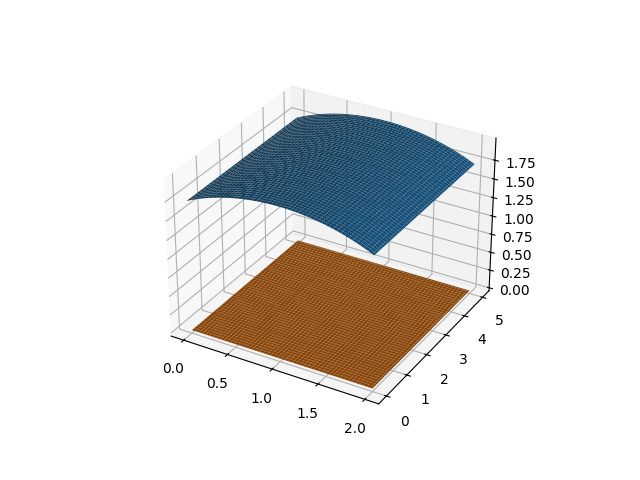
\includegraphics[width=0.8\linewidth]{cylinder.png}
\caption[]{}
\label{fig:cylinder}
Поверхность z(x, y) (\ref{eq:surfcyl}).	% chktex 36
\end{figure}

Возьмём подынтегральную функцию $f(x,y) = 1$, тогда значение интеграла легко вычисляется аналитически:

\begin{equation}
I = \frac{2 \pi R}{3} = 10.471975512
\end{equation}

В таблице (\ref{table:cylinder}) представлены значения поверхностного интеграла, вычисленного методом триангуляции на сетках с различным числом узлов.

\begin{table}[ht]
\centering
\begin{tabular}{|c|c|c|c|c|}
\hline
 Число узлов	& 50		& 100		& 200		& 400		\\ 
\hline
 Значение $I_h$		& 10,471783	& 10,471927	& 10,471963	& 10,471972	\\  
\hline
\end{tabular}
\caption{Зависимость значения $I_h$ от числа узлов\label{table:cylinder}}
\end{table}

Абсолютная погрешность вычисленного поверхностного интеграла на сетках с различным числом точек для поверхности, заданной уравнением (\ref{eq:surfcyl}), представлена в таблице \ref{table:abspogcylinder}.

\begin{table}[ht]
\centering
\begin{tabular}{|c|c|c|c|c|}
\hline
 Число узлов			& 50					& 100					& 200					& 400		\\ 
\hline
 Абсолютная погрешность & $1.92 \cdot 10^{-4}$	& $4,81 \cdot 10^{-5}$	& $1,20 \cdot 10^{-5}$	& $3,01 \cdot 10^{-6}$	\\  
\hline
\end{tabular}
\caption{\label{table:abspogcylinder}}
Абсолютная погрешность для интеграла, вычисленного описанным методом триангуляции.
\end{table}

Из соотношения (\ref{eq:runge1})
\begin{align}\label{eq:runge2}
m = \log_2(\frac{I_{\frac{h}{2}}-I_{h}}{I-I_{\frac{h}{2}}}+1) = \notag \\ 
= \log_2(\frac{I-I_{h}}{I-I_{\frac{h}{2}}})
\end{align}

В таблице \ref{table:porTochCylinder} представлены значения порядка точности вычисления поверхностного интеграла на сгущающихся в два раза сетках.

\begin{table}[ht]
\centering
\begin{tabular}{|c|c|c|c|}
\hline
 Число узлов		& 50 $\rightarrow$ 100	& 100 $\rightarrow$ 200	& 200 $\rightarrow$ 400	\\ 
\hline
 Порядок точности $m$	& 2.029272	& 2.014531	& 2.007240	\\  
\hline
\end{tabular}
\caption{\label{table:porTochCylinder}}
Порядок точности в зависимости от числа узлов сетки, вычисленные методом Рунге.
\end{table}

Порядок точности представленного выше метода вычисления поверхностного интеграла.

\subsubsection*{Тест 2}

Рассмотрим поверхность вида $z(x,y)$ (\ref{eq:surfcy2})

\begin{equation}\label{eq:surfcy2}
z = x^2
\end{equation}

\begin{figure}[H]
\centering
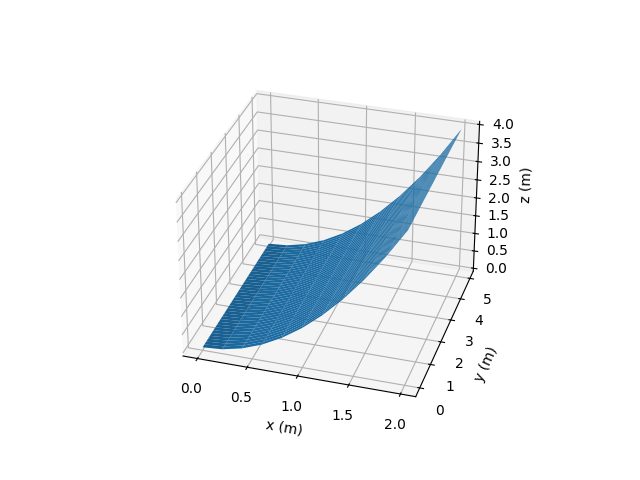
\includegraphics[width=0.8\linewidth]{squareSurf.png}
\caption[]{}
\label{fig:squareSurf}
Поверхность вида (\ref{eq:surfcy2})
\end{figure}

Аналитическое значение интеграла считается элементарно:

\begin{equation}
I = 23.233919
\end{equation}

Значения, посчитанные методом триангуляции, показаны в таблице \ref{table:square}.

\begin{table}[ht]
\centering
\begin{tabular}{|c|c|c|c|c|}
\hline
 Число узлов	& 50		& 100		& 200		& 400		\\ 
\hline
 Значения		& 23.233245	& 23.233754	& 23.233878	& 23.233909	\\  
\hline
\end{tabular}
\caption{\label{table:square}}
Приближенные значения интеграла, полученные вышеописанным методом.
\end{table}

Порядок точности $m$ посчитаются по формуле (\ref{eq:runge2}) и представлены в таблице \ref{tablee:porTochSquare}.

\begin{table}[ht]
\centering
\begin{tabular}{|c|c|c|c|}
\hline
 Число узлов		& 50 - 100	& 100 - 200	& 200 - 400	\\ 
\hline
 Порядок точности	& 2.029296	& 2.014537	& 2.007242	\\  
\hline
\end{tabular}
\caption{\label{tablee:porTochSquare}}
Порядок точности в зависимости от числа узлов сетки, вычисленные методом Рунге.
\end{table}

Порядок точности второй, аналогично тесту с поверхностью, заданной уравнением (\ref{eq:surfcyl}).

Из анализа таблиц 1–5 следует, что предложенный в работе метод вычисления площади поверхности имеет второй порядок точности.

\section{Численное исследование значений управляющих параметров в электролизной ванне для МГД-стабильных и МГД-нестабильных режимов работы электролизной ванны}

Поскольку для эффективного управления ванной при помощи АСУТП необходимо знать значения параметров выхода по току и потери выхода по току, представляет интерес приведение численного расчета значений этих параметров при помощи разработанного выше метода. Ниже приводятся результаты численного исследования значений выхода по току и потерь выхода по току для МГД-стабильных и нестабильных режимов работы ванны.

\subsection{Исследование выхода по току и потерь по току в случае МГД-стабильного режима работы ванны.}

При помощи расчета основного математического комплекса при МГД-стабильном режиме работы ванны проведем вычисление значений выхода по току при помощи формул (\ref{eq1}) и (\ref{eq:modeq2}).

\begin{figure}[H]
\centering
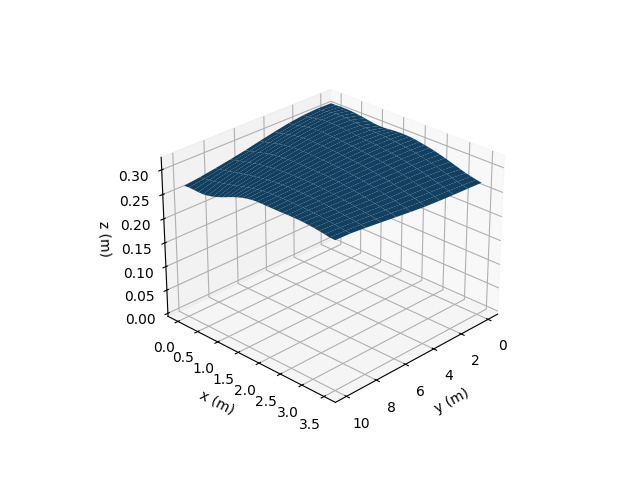
\includegraphics[width=0.8\linewidth]{h.png}
\caption{Граница раздела сред металл-электролит в момент времени $t_1$ при МГД-стабильном режиме работы. \label{fig:hsurf}}
\end{figure}

Оценим выход по току, используя формулу (\ref{eq1}). Размер ванны $3.4 m$ на $9.4 m$, площадь анодов $15.876 m^2$, температура $950 C^{\circ}$, МПР $0.0315 m$, $i_a = 3 \frac{A}{m^2}$.

\begin{equation}
\eta=(1-2567 \cdot \frac{15.876^{0,21}}{3^{0.58} \cdot 0.0314 \cdot e^{\frac{12940}{950}}}) \cdot 100 = 90.646 \%
\end{equation}

По модифицированной формуле (\ref{eq:modeq2}) получим значения потерь по току:

\begin{equation}
\Delta \eta = 0.00674
\end{equation}

На рисунке 20 изображена поверхность в момент времени $t_2 > t_1$. Наглядно видно, что за время $\Delta t$ поверхность немного выровнялась, при этом минимальное значение МПР увеличилось, а максимальное уменьшилось. Оценим, как изменились выход и потери по току.

\begin{figure}[H]
\centering
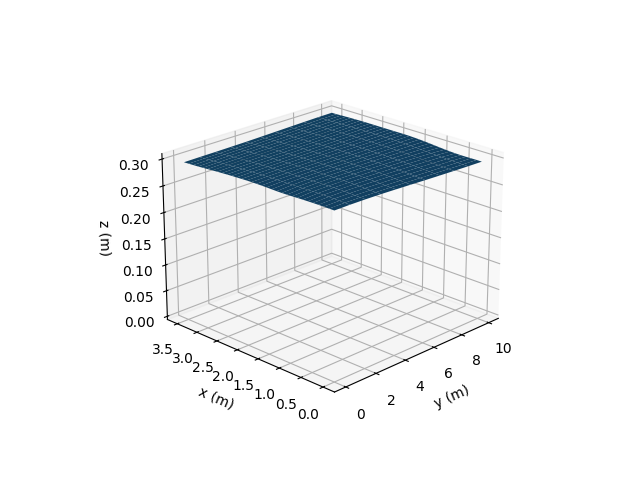
\includegraphics[width=0.8\linewidth]{h2.png}
\caption{Граница раздела сред металл-электролит в момент времени $t_2$ при МГД-спокойствии. \label{fig:hsurf-}}
\end{figure}

Для границы раздела сред в момент времени $t_2$ выход по току и потери по току \ref{eq:vichpotoku22}, \ref{eq:poterupotoku22}.

\begin{equation}\label{eq:vichpotoku22}
\eta=(1-2567 \cdot \frac{15.876^{0,21}}{0.688^{0.58} \cdot 0.0815 \cdot e^{\frac{12940}{960}}}) \cdot 100 = 93.594 \%
\end{equation}

\begin{equation}\label{eq:poterupotoku22}
\Delta \eta = 0.00667
\end{equation}

Изменение выхода по току и потерь выхода по току показывает существенную зависимость выхода по току от формы границы раздела.

Величина $\eta$ увеличилась на $2.048\%$, величина $\Delta \eta$ уменьшилась на $0.007$, что соответствует $1.038\%$ выхода по току.

Значения величин выхода по току и потерь по току объясняется тем, что обе не являются точными, и параметры, по которым они вычисляются, несмотря на свою взаимозависимость, являются существенно разными и определяются с различными погрешностями.

\subsection{Исследование значений управляющих параметров ванны в состоянии МГД-нестабильности при выемке анодов.}

Во время работы электролизной ванны нередко возникает состояние МГД-нестабильности, например, при одновременной замене 11-го и 22-го анодов. При этом на границе раздела имеет большую амплитуду возмущения, расстояние между катодом и анодом становится малым и может привести к его выходу из строя.

На рисунке \ref{fig:anodout} показана поверхность раздела сред при выемке анодов.

\begin{figure}[H]
\centering
\includegraphics[width=0.8\linewidth]{Surf1.png}
\caption{Граница раздела сред металл-электролит при выемке анодов в момент времени $t_1$. \label{fig:anodout}}
\end{figure}

Оценим выход по току, используя формулу (\ref{eq1}). Размер ванны $3.5 m$ на $10 m$, площадь анодов $17.5 m^2$, температура $960 C^{\circ}$, МПР $0.05 m$, $i_a = 0.5 \frac{A}{m^2}$.
\begin{equation}
\eta=(1-2567 \cdot \frac{17.5^{0,21}}{1.5^{0.58} \cdot 0.05 \cdot e^{\frac{12940}{960}}}) = 89.638 \%
\end{equation}

Без моделирования поверхности раздела в реальном времени невозможно предсказать, в какой точке ванны будут достигаться минимальный и максимальный МПР. Выбор конкретного места проведения замера МПР проводится из соображений физической возможности добраться до нужного места при взятии проб, при этом выбор конкретного места нередко может приниматься непосредственно перед замером вне зависимости от происходящих в ванне процессов. Таким образом, место замера может быть случайно выбрано в месте максимального МПР. В таком случае, применив полуэмпирическую формулу (\ref{eq2}), получим результат:

\begin{equation}
\Delta \eta = 0.0074
\end{equation}


Воспользовавшись методом триангуляции, посчитаем потерю по току по модифицированной формуле (\ref{eq:modeq2}).

\begin{equation}
\Delta \eta = 0.0139
\end{equation}

Для того, чтобы оценить изменение потери по току, возьмём другое состояние этой же ванны в момент времени $t_2$.

\begin{figure}[H]
\centering
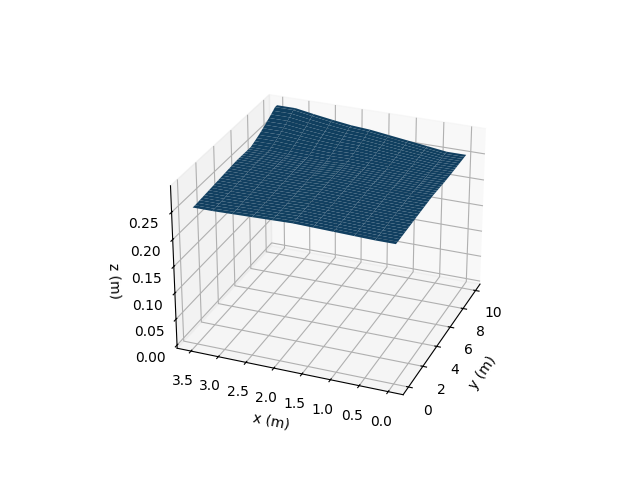
\includegraphics[width=0.8\linewidth]{Surf2.png}
\caption{Ганица раздела сред металл-электролит при выемке анодов в момент $t_2$ \label{fig:anodout-}}
\end{figure}

Момент времени $t_2$ соответствует процессу восстановления МГД-стабильности после замены анода. Всплеск в большей степени выровнялся, что привело к уменьшению максимального МПР и увеличению минимального. Оценим выход по току по формуле (\ref{eq1}) для поверхности (\ref{fig:anodout-}):

\begin{equation}
\eta=(1-2567 \cdot \frac{17.5^{0,21}}{1.5^{0.58} \cdot 0.07 \cdot e^{\frac{12940}{960}}}) = 91.365 \%
\end{equation}

Посчитаем потери по току для максимального МПР по эмпирической формуле (\ref{eq2}):

\begin{equation}
\Delta \eta = 0.0099
\end{equation}

По модифицированной формуле (\ref{eq:modeq2}) вычислим потери по току:

\begin{equation}
\Delta \eta = 0.0107
\end{equation}

Таким образом $\eta$ изменился на $1.727\%$, тогда как $\Delta \eta$ изменился на $0.00017$, что соответвстует $1.799\%$

Значениями формул (\ref{eq1}) и (\ref{eq:modeq2}) дают очень похожий результат изменения выхода по току, даже несмотря на погрешности параметров, от которых они зависят. Также стабильно остаётся тренд на увеличение выхода по току при переходе к более спокойной поверхности.

При этом немодифицированная формула (\ref{eq2}) для измерения в точке максимального МПР противоречит тренду на увеличение выхода по току. С точки зрения процессов, происходящих в ванне, неравномерное распределение металла в электролизёре ведёт к неравномерному распределению тока по ванне, перемешиванию алюминия и электролита, опасности короткого замыкания, что, соответственно, приводит к уменьшению полезной работы тока, обратному окислению алюминия или даже полному выходу из строя электролизёра. В совокупности эти последствия значительно уменьшают итоговый выход по току или полную остановку процесса электролиза. Таким образом, тренд на уменьшение выхода по току по формуле (\ref{eq2}) при ослаблении возмущений поверхности раздела противоречит природе происходящих процессов. В свою очередь, модифицированная формула (\ref{eq:modeq2}) лишена этого недостатка.

\subsection{Исследование значений управляющих параметров ванны во время анодного эффекта.}

Существенное ухудшение смачиваемости анода электролитом приводит к анодному эффекту, который сопровождается резким поднятием напряжения на электролизере. Выделяются пузырьки газа, увеличивается поверхностное натяжение электролита, что негативно сказывается на выходе алюминия по току. Посчитаем управляющий параметр выхода по току на данных, приведенных в диссертации~\cite{litlink:kalmykov}, и продемонстрированных на рисунке \ref{fig:anodeffect}.

\begin{figure}[H]
\centering
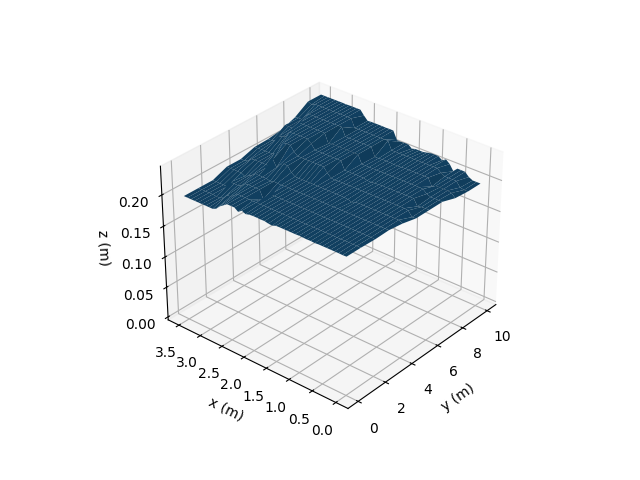
\includegraphics[width=0.8\linewidth]{anodeffect.png}
\caption{Граница раздела сред металл-электролит при анодном эффекте в момент времени $t_1$ \label{fig:anodeffect}}
\end{figure}

Рассчитаем выход по току и потери по току для поверхности при анодном эффекте:

\begin{equation}
\eta=(1-2567 \cdot \frac{17.5^{0,21}}{1.5^{0.58} \cdot 0.04 \cdot e^{\frac{12940}{960}}}) = 87.048 \%
\end{equation}

\begin{equation}
\Delta \eta = 0.01188
\end{equation}


Возьмём момент времени $t_2$, соответствующий границе раздела сред после окончания процессов анодного эффекта. Полученная поверхность продемонстрирована на рисунке \ref{fig:anodeffect-}.

\begin{figure}[H]
\centering
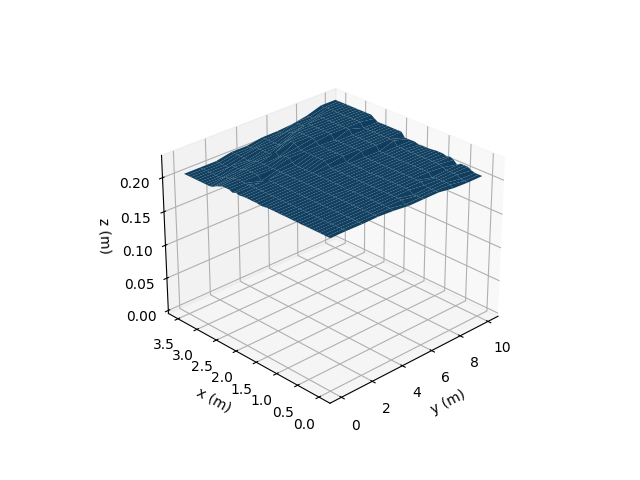
\includegraphics[width=0.8\linewidth]{anodeffect-.png}
\caption{Граница раздела сред металл-электролит при анодном эффекте в момент времени $t_2$ \label{fig:anodeffect-}}
\end{figure}

\begin{equation}
\eta=(1-2567 \cdot \frac{17.5^{0,21}}{1.5^{0.58} \cdot 0.052 \cdot e^{\frac{12940}{960}}}) = 90.037 \%
\end{equation}

\begin{equation}
\Delta \eta = 0.01173
\end{equation}

Исследуем изменение этих величин:

\begin{equation}
90.037 - 87.048 = 2.989 \%
\end{equation}

\begin{equation}
(0.01188 - 0.01173) \cdot 100 = 0.015 \%
\end{equation}

Величина $\eta$ увеличилась на $2.989\%$, величина $\Delta \eta$ уменьшилась на $0.015$, что соответствует $1.262\%$ выхода по току.

Таким образом, наблюдается корреляция выхода по току, то есть при увеличении выхода по току уменьшаются потери выхода по току и наоборот, при уменьшении выхода по току увеличиваются потери по току.

Несовпадение процентного выхода по току объясняется тем, что соответствующие величины определяются набором данных, которые соответствуют своему набору параметров, которые также измеряются с погрешностью.

\subsection{Объединение полученных данных.}

Ниже приведены полученные в предыдущих разделах значения в удобной для анализа форме.

\begin{table}[ht]
\centering
\begin{tabular}{|c|c|}
\hline
			&Выход по току	\\
\hline
Поверхность при МГД стабильности &	\\
Рис. \ref{fig:hsurf} (момент времени $t_1$)			&90.646	\\ 
Рис. \ref{fig:hsurf-} (момент времени $t_2$)		&93.594	\\  
\hline
Поверхность при выемке анодов &	\\
Рис. \ref{fig:anodout} (момент времени $1_1$)		&89.638	\\  
Рис. \ref{fig:anodout-} (момент времени $t_2$)		&91.365	\\  
\hline
Поверхность при анодом эффекте &	\\
Рис. \ref{fig:anodeffect} (момент времени $t_1$)	&87.048	\\  
Рис. \ref{fig:anodeffect-} (момент времени $t_2$)	&90.037	\\  
\hline
\end{tabular}
\caption{Выход по току $\eta$. \label{table:vichPoToku}}
\end{table}

\begin{table}[ht]
\centering
\begin{tabular}{|c|c|}
\hline
			&Потери по току	\\
\hline
Поверхность при МГД стабильности &	\\
Рис. \ref{fig:hsurf} (момент времени $t_1$)			&0.00674\\ 
Рис. \ref{fig:hsurf-} (момент времени $t_2$)		&0.00667\\  
\hline
Поверхность при выемке анодов &	\\
Рис. \ref{fig:anodout} (момент времени $t_1$)		&0.00928\\  
Рис. \ref{fig:anodout-} (момент времени $t_2$)		&0.00945\\  
\hline
Поверхность при анодом эффекте &	\\
Рис. \ref{fig:anodeffect} (момент времени $t_1$)	&0.01188\\  
Рис. \ref{fig:anodeffect-} (момент времени $t_2$)	&0.01173\\  
\hline
\end{tabular}
\caption{Потери по току $\Delta \eta$. \label{table:poteriPoToku}}
\end{table}

\begin{table}[ht]
\centering
\begin{tabular}{|c|c|}
\hline
			& Изменение выхода по току (\%) \\
			& $\eta(t_2)-\eta(t_1)$		\\
\hline
Поверхность при МГД стабильности &	\\
Рис. \ref{fig:hsurf} и \ref{fig:hsurf-}			&2.948\\ 
\hline
Поверхность при выемке анодов &	\\
Рис. \ref{fig:anodout} и \ref{fig:anodout-}		&1.727\\ 
\hline
Поверхность при анодом эффекте &	\\
Рис. \ref{fig:anodeffect} и \ref{fig:anodeffect-}&2.989\\ 
\hline
\end{tabular}
\caption{Изменение выхода по току. \label{table:ismineniev}}
\end{table}

\begin{table}[ht]
\centering
\begin{tabular}{|c|c|c|}
\hline
			& Изменение потерь по току & Изменение потерь по току (\%)\\
			& $\Delta \eta(t_1) - \Delta \eta(t_2)$ & - \\
\hline
Поверхность при МГД стабильности & &	\\
Рис. \ref{fig:hsurf} и \ref{fig:hsurf-}			&0.00007 & 1.038\\ 
\hline
Поверхность при выемке анодов & &	\\
Рис. \ref{fig:anodout} и \ref{fig:anodout-}		&0.0032 & 1.799\\ 
\hline
Поверхность при анодом эффекте & &	\\
Рис. \ref{fig:anodeffect} и \ref{fig:anodeffect-}&0.00015 & 1.262\\ 
\hline
\end{tabular}
\caption{Изменение потерь по току. \label{table:ismineniep}}
\end{table}

Несмотря на то, что абсолютные значения изменения выхода по току и изменения потерь по току сильно отличаются, они имеют общую тенденцию на уменьшение выхода по току при искривлении поверхности. Такой результат можно было ожидать, поскольку формулы зависят от совершенно разных параметров, сильно связанных между собой в электролизёре, но независимых в приведённом расчёте. Так, например, при возникновении анодного эффекта из-за пузырьков газа повышается температура в электролизёре, а выемка анода в электролизёре приводит к перераспределению тока в ванне, и распределение силы тока становится сильно неравномерным. В приведённом расчёте нет возможности учесть эти взаимодействия, в итоге при изменении формы поверхности температура считается неизменной, что сильно сказывается на формуле (\ref{eq1}). Тем не менее общие тенденции, как уже было сказано, зафиксировать можно.

\newpage
\section{Численное вычисление распределения потерь по току в случае нестабильного и стабильного режимов работы ванны.}

Поскольку формула (\ref{eq2}) представляет из себя поверхностный интеграл, она позволяет получить распределение потерь по току по горизонтальному срезу ванны. Распределение потерь по току наглядно показано на рисунках \ref{fig:raspStab}, \ref{fig:raspAnodOut}, \ref{fig:raspAnod} для поверхностей \ref{fig:hsurf}, \ref{fig:anodout} и \ref{fig:anodeffect} соответственно. Множитель $\mu = 10^{-6}$.

\begin{figure}[H]
\centering
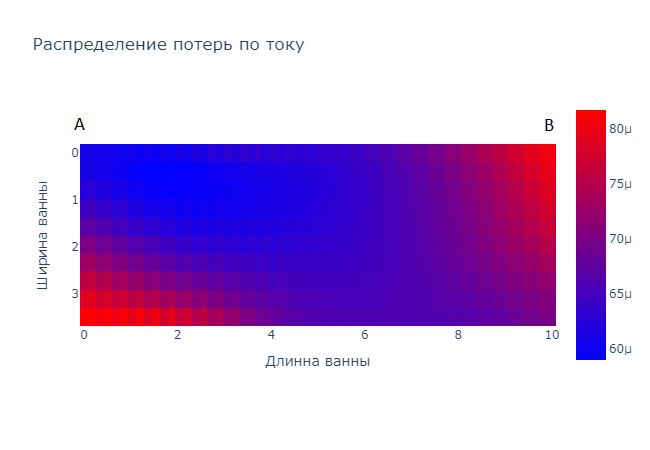
\includegraphics[width=0.8\linewidth]{hloss.png}
\caption{Распределение потерь по току в ванне в стабильном состоянии.\label{fig:raspStab}}
\end{figure}

\begin{figure}[H]
\centering
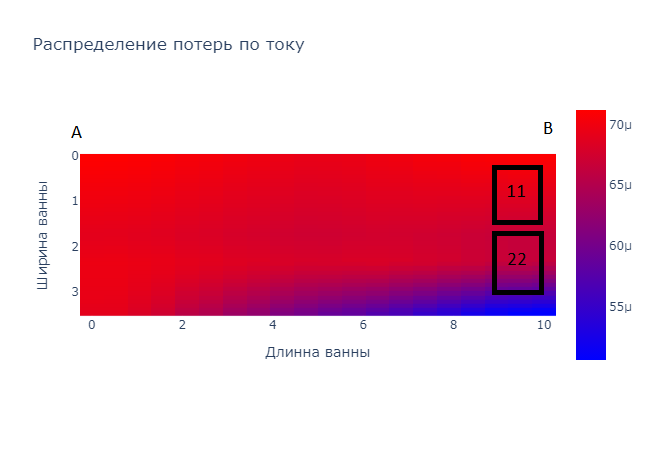
\includegraphics[width=0.8\linewidth]{surfloss.png}
\caption{Распределение потерь по току в ванне выемке 11 и 22 анодов.\label{fig:raspAnodOut}}
\end{figure}

\begin{figure}[H]
\centering
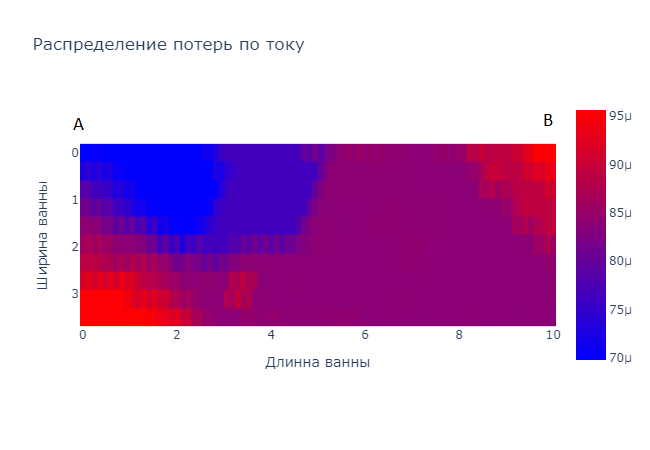
\includegraphics[width=0.8\linewidth]{anodloss.png}
\caption{Распределение потерь по току в ванне при анодном эффекте.\label{fig:raspAnod}}
\end{figure}

Измерения МПР проводятся вдоль борта АВ, как правило, берется лишь одно измерение посередине ванны. Для МГД-стабильного режима работы ванны и случая выемки анодов такое измерение действительно даст представление о характере происходящих процессов и позволит принять соответствующие меры, однако в случае анодного эффекта результат измерения может сильно варьироваться в зависимости от выбранной точки измерения, что может ввести в заблуждение и привести к увеличению потерь по току или даже выходу электролизера из строя.

Проведенное в работе исследование позволяет дать рекомендации по измерению МПР в промышленной ванне с целью определения МГД-стабильности работы ванны, что, в свою очередь, позволяет внести корректировки в АСУТП электролизной ванны и приведет к более эффективному режиму управления, соответствующему повышению выхода алюминия по току.

\section*{Заключение}
\addcontentsline{toc}{section}{Заключение}

Электролиз алюминия - сложный и комплексный процесс. Для оценки его эффективности нельзя опираться только на прибыль или количество полученного продукта, поскольку рыночная цена металла может колебаться, мало завися от эффективности конкретного производства, а увеличение количества получаемого алюминия может достигаться за счёт больших потерь тепловой энергии, из-за чего может падать прибыльность. Чтобы оценить эффективность технологического процесса, предлагается использовать выход по току. Этот параметр не зависит от рыночных показателей и учитывает расход энергии на поддержание процесса электролиза.

Для оценки параметра выхода по току в литературе были найдены полуэмпирическая и теоретическая формулы (\ref{eq1}), (\ref{eq2}). Был проведён анализ этих формул, проведены вычисления значений на тестовых примерах. По результатам анализа была предложена модифицированная формула (\ref{eq:modeq2}), учитывающая большее количество данных и не опирающаяся на усреднение МПР.

Для вычисления поверхностных интегралов, использующихся в формулах (\ref{eq2}) и (\ref{eq:modeq2}), в данной работе был разработан метод простой триангуляции, позволяющий в реальном времени и с хорошей точностью получать значения потерь выхода по току. Было проведено исследование точности разработанного метода на практике.

В работе также был приведён сравнительный анализ значений управляющих параметров, полученных формулами (\ref{eq1}), (\ref{eq2}), с помощью разработанного метода триангуляции при различных состояниях процесса электролиза в ванне. Рассматривались как состояния спокойствия, так и состояния МГД-нестабильности, а именно возмущения при выемке анодов и анодный эффект. Помимо этого, было оценено распределение потерь по току при этих процессах ванны.

\subsubsection*{Основные результаты}

\begin{enumerate}
	\item Предложен алгоритм расчета площади криволинейной поверхности на основе метода триангуляции. Исследована сходимость метода на сгущающихся сетках.

	\item Предложена модифицированная формула вычисления величины потерь по току, проведена ее верификация.

	\item Реализовано численное вычисление значений выхода по току и потерь выхода по току, показана корреляция этих управляющих параметров.

	\item Численно исследованы распределения потерь по току в планарной плоскости разреза ванны для МГД-стабильной работы ванны, работы ванны и для МГД-нестабильной работы ванны в случае выемки двух анодов и анодного эффекта.

	На основе проведенных численных исследований были выработаны рекомендации по управлению работой ванны.
\end{enumerate}


\newpage
 
% даём указание на включение данного места в оглавление как секции (\section)
\addcontentsline{toc}{section}{Список литературы}
 
%далее сам список используевой литературы
\begin{thebibliography}{}
	\bibitem{litlink:kalmykov} Калмыков А.В. Математическое моделирование влияния процессов тепломассопереноса на МГД-стабильность алюминиевого электролизёра // Москва: Московский государственный университет имени М.В. Ломоносова. Факультет вычислительной математики и кибернетики. Кафедра вычислительных методов. Диссертация. 2017.
	\bibitem{litlink:bibliogr}  Белолипецкий В. М., Пискажова Т.В. Математическое моделирование процесса электролитического получения алюминия. Решение задач управления технологией // Красноярск: Сибирский федеральный университет. Библиогр. 2013.
	\bibitem{litlink:derkach} Деркач А.С., Левитан Г.У., Лебедев В.И., Сенин В.Н., Солнцев С.С., Форсблом Г.В. Электролиз алюминия // Издательство 'Металлургия' Москва 1966.
	\bibitem{litink:AE} Grjotheim K., Rrohn C., Malinovsky. M., Matiasovsky K., Thonstad J. 2nd Edition Aluminium Electrolysys. Fundamentals of the Hall-Heroult Process. // Dusseldorf 1982.
	\bibitem{litlink:VAMI} Тепловые процессы в электролизерах и миксерах алюминиевого производства. / Под общей редакцией Громова Б. С., М.: – 1998. – С. 322.
	\bibitem{litlink:korobov} Коробов, М. А. Самообжигающиеся аноды алюминиевых электролизеров / М. А. Коробов, А. А. Дмитриев // М.: Металлургия. – 1972. – 207 с.
	\bibitem{litlink:Lillebuen}Lillebuen, B. Current Efficiency and back reaction in aluminium electrolysis // Electrochim. Acta. – 1980, V25. – P. 131– 137. 
	\bibitem{litlink:derkach2}Деркач, А. С. Влияние нестабильности тока серии на технологический режим алюминиевых электролизеров// Цветные металлы. – 1967. – № 3. – С. 39– 40.
	\bibitem{litlink:Kudryavcev}Кудрявцев Л.Д. Курс математического анализа. Том 2. // Дрофа 2004
	\bibitem{litlink:scvortsov}  Скворцов А.В., Мирза Н.С. Алгоритмы построений и анализа триангуляции // 'Издательство томского университета' 2006.
	\bibitem{litlink:shirok} Широкий А.А., Аппроксимационные свойства триангуляций поверхностей // Казань 2012.
	\bibitem{litlink:samarskiy} Самарский А.А. Гулин А.В. Численные методы // Москва 'Наука' 1989
\end{thebibliography}

\end{document}
